% Vorlage für eine Bachelorarbeit
% Siehe auch LaTeX-Kurs von Mathematik-Online
% www.mathematik-online.org/kurse
% Anpassungen für die Fakultät für Mathematik
% am KIT durch Klaus Spitzmüller und Roland Schnaubelt Dezember 2011

\documentclass[12pt,a4paper]{scrartcl}
% scrartcl ist eine abgeleitete Artikel-Klasse im Koma-Skript
% zur Kontrolle des Umbruchs Klassenoption draft verwenden


% die folgenden Packete erlauben den Gebrauch von Umlauten und ß
% in der Latex Datei
\usepackage[utf8]{inputenc}
% \usepackage[latin1]{inputenc} %  Alternativ unter Windows
\usepackage[T1]{fontenc}
\usepackage[ngerman]{babel}


\usepackage[pdftex]{graphicx}
\usepackage{latexsym}
\usepackage{amsmath,amssymb,amsthm}
\usepackage{setspace}
\usepackage{url}
\usepackage{mathtools}
\usepackage{enumitem}
\usepackage{float}


% Abstand obere Blattkante zur Kopfzeile ist 2.54cm - 15mm
\setlength{\topmargin}{-15mm}


% Umgebungen für Definitionen, Sätze, usw.
% Es werden Sätze, Definitionen etc innerhalb einer Section mit
% 1.1, 1.2 etc durchnummeriert, ebenso die Gleichungen mit (1.1), (1.2) ..
\theoremstyle{definition}
\newtheorem{Satz}{Satz}[section]
\newtheorem{Folgerung}[Satz]{Folgerung} 
\newtheorem{Definition}[Satz]{Definition} 
\newtheorem{Lemma}[Satz]{Lemma}		   
                  
\numberwithin{equation}{section} 

\newtheorem*{Bemerkung}{Bemerkung}

% einige Abkuerzungen
\newcommand{\C}{\mathbb{C}} % komplexe
\newcommand{\K}{\mathbb{K}} % komplexe
\newcommand{\R}{\mathbb{R}} % reelle
\newcommand{\Q}{\mathbb{Q}} % rationale
\newcommand{\Z}{\mathbb{Z}} % ganze
\newcommand{\N}{\mathbb{N}} % natuerliche

% eigene Definitionen
\newcommand{\dx}{\, \mathrm{d} x}
\newcommand{\da}{\, \mathrm{d} a}
\newcommand{\dt}{\, \mathrm{d} t}
\newcommand{\ds}{\, \mathrm{d} s}
\newcommand{\dP}{\, \mathrm{d} \mathbb{P}}
\newcommand{\icol}[1]{%inline row vector
		\left(	\begin{smallmatrix}#1\end{smallmatrix} \right) %
	}
\newcommand{\abs}[1]{| #1 |}
\newcommand{\ubar}[1]{\underline{#1}{}}
\DeclareMathOperator{\dive}{div}
\DeclareMathOperator{\spann}{span}
\DeclareMathOperator{\conv}{conv}
\DeclareMathOperator{\supp}{supp}

\begin{document}
  % Keine Seitenzahlen im Vorspann
  \pagestyle{empty}
  
  
  % Titelblatt der Arbeit
  \begin{titlepage}

    
\includegraphics[scale=0.45]{kit-logo.jpg} 
    \vspace*{2cm} 

 \begin{center} \large 
    
    Bachelorarbeit
    \vspace*{2cm}

    {\huge Die Multilevel Monte Carlo Methode und deren Anwendung am Beispiel der linearen Transportgleichung}
    \vspace*{2.5cm}

    Tim Buchholz
    \vspace*{1.5cm}

    ??.??.??
    \vspace*{4.5cm}


    Betreuung: Prof.Dr. Christian Wieners und M.Sc. Niklas Baumgarten \\[1cm]
    Fakultät für Mathematik \\[1cm]
		Karlsruher Institut für Technologie
  \end{center}
\end{titlepage}



  % Inhaltsverzeichnis
  \tableofcontents

\newpage
 


  % Ab sofort Seitenzahlen in der Kopfzeile anzeigen
  \pagestyle{headings}

\section{Einleitung}
% !TeX root = bachelorarbeit.tex

\section{Einleitung}

Monte Carlo Methoden sind weit verbreitet, um in unterschiedlichsten Situationen Erwartungswerte stochastischer Modelle zu schätzen.
So werden bei der Monte Carlo Quadratur, der wohl bekanntesten Anwendungen der Monte Carlo Methode, zufällig gleichverteilte Stützstellen dafür genutzt, den Erwartungswert der Funktionsauswertung an einer zufälligen Stützstelle zu bestimmen. Daraus lässt sich anschließend der approximierte Integralwert auf einer gegebenen Grundmenge bestimmen. 
Wir wollen Monte Carlo Methoden dazu nutzen, eine stochastische partielle Differentialgleichung zu lösen. 
Genauer betrachten wir eine stochastisch beeinflusste Zielgröße $ Q $ der Lösung der Differentialgleichung und fragen uns, welchen Wert $ \mathbb{E}[Q] $ nimmt $ Q $ im Mittel an? Wir suchen also nach einem Erwartungswert, was die Verwendung von Monte Carlo Methoden zumindest einmal nahelegt. 
Außerdem wollen wir uns dabei die Vorteile der sogenannten Multilevel Monte Carlo (MLMC) Methode zunutze machen. Diese wurde zunächst von Heinrich für Approximation von parameterabhängigen Integralen in hohen Dimensionen entwickelt (vgl. \cite{heinrich2001multilevel}) und anschließend unter anderem von  Giles auf stochastisch modellierte partielle Differentialgleichungen übertragen. Folgendes Zitat bringt die Vorteile auf den Punkt, welche die Multilevel Monte Carlo Methode in diesem Zusammenhang bietet:
\begin{quote}
	\textit{Monte Carlo methods are a very general and useful approach for the estimation of expectations arising from stochastic simulation. However, they can be computationally expensive, particularly when the cost of generating individual stochastic samples is very high, as in the case of stochastic PDEs. \\ Multilevel Monte Carlo is a recently developed approach which greatly reduces the computational cost by performing most simulations with low accuracy at a correspondingly low cost, with relatively few simulations being performed at high accuracy and a high cost.}  \\
	\rightline{Michael B. Giles in \cite{giles_2015}. \, \qquad \qquad }
\end{quote}
Das Lösen, bzw. in unserem Fall das Bestimmen eines Erwartungswert, von stochastisch modellierten partiellen Differentialgleichungen fallen in das Gebiet der Uncertainty Quantification. Dieses noch recht 'junge' Feld der Mathematik wird von Sullivan in \cite{sullivan2015introduction} als ein 'Zusammentreffen der Wahrscheinlichkeitstheorie, Numerik, Statistik und der echten Welt' beschrieben. \\
Die Thesis lässt sich aktuellen Arbeiten am Institut für Angewandte und Numerische Mathematik, wie etwa \cite{BAUMGARTEN2020}, zuordnen und soll daher zwar zum einen den theoretischen Hintergrund darlegen, aber auch einige Ergebnisse präsentieren, die im parallelen Finite Elemente System M++ \cite{siteM++} erzielt werden konnten, welches am Institut für Angewandte und Numerische Mathematik unter anderem von Herrn Prof. Dr. C. Wieners entwickelt wurde. \\
Konkret wollen wir vor allem die zeitabhängige lineare Transportgleichung betrachten. Dabei handelt es sich um ein weit verbreitetes Modellproblem, welches unter Anderem auch in \cite{di2011mathematical}, einem Standardwerk für Discontinuous Galerkin Methoden, zu finden ist. 
Dabei nutzen wir wie in \cite{di2011mathematical} die sogenannte 'method of lines': Zur numerischen Lösung der Differentialgleichung nutzen wir ein Discontinuous Galerkin Verfahren (DGV) im Ort und kombinieren diese zunächst semidiskrete Lösung mit einem geeigneten Zeitschrittverfahren. Aufgrund der Wahl eines Runge-Kutta Verfahrens erhalten wir somit ein Runge-Kutta Discontinuos Galerkin Verfahren. Einen Überblick über diese Verfahrensart findet man zum Beispiel auch in \cite{cockburn2001runge}.
Ebenfalls mit der Anwendung von Multilevel Monte Carlo Methoden auf eine Variante des Transportproblems mit Diffusion haben sich zum Beispiel auch Barth und Stein in \cite{barth2013multilevel} bzw. \cite{barth2019multilevel} oder Kumar et al. in \cite{kumar2018multigrid} beschäftigt. Mit Multilevel Monte Carlo Methoden im Allgemeinen haben sich neben den bereits erwähnten Giles und Barth auch Cliffe in \cite{cliffe2011multilevel}, Charrier in \cite{charrier2012strong} oder Teckentrup in \cite{teckentrup2013further}, um nur Einige zu nennen, befasst.
Um die eigentliche Idee der Multilevel Monte Carlo Methode in den Vordergrund zu rücken, wollen wir diese aber auch wie in \cite{heinrich2001multilevel} am Beispiel der numerischen Integration betrachten.
Dabei wollen wir insbesondere die Unterschiede zu und Vorteile gegenüber der Standard Monte Carlo Methode hervorheben, welche im Kern bereits durch obiges Zitat zusammengefasst sind.

%Monte Carlo Methoden sind weit verbreitet und finden in verschiedenen Bereichen der Mathematik ihre Anwendung.
%Sie dienen dabei als statistische Schätzer für Erwartungswerte. 
%Eine der bekanntesten Anwendungen ist wohl die Monte Carlo Quadratur, welche zur numerischen Integration genutzt werden kann.
% 
%Nachdem Giles (cite ...) ... gewöhnliche DGL ... kam ... für SPDE's zu nutzen ...cite .
%
%
%Allerdings besitzt die Monte Carlo Methode einen entscheidenden Nachteil, will man sie im Zusammenhang unsicherer Ausgangsdaten für die Lösung von partiellen Differentialgleichungen nutzen, sie konvergiert im Normalfall relativ langsam und das numerische Lösen von PDE's ist oft sehr aufwendig.
%Es werden also unter Umständen sehr viele, sehr teure Zufallssamples benötigt, um ein vernünftiges Ergebnis zu erhalten. \newline
%Diese Thesis soll sich daher mit der Multilevel Monte Carlo Methode (im Folgenden MLMC Methode genannt) beschäftigen, welche an die Monte Carlo Methode angelehnt ist, aber durch die geschickte Auswertung der (Zufalls-Samples) deutliche Effizienzvorteile gegenüber der Standard Monte Carlo Methode besitzt.
%Die MLMC Methode soll nach einer ausführlichen theoretischen Analyse auch praktisch auf das Transportproblem angewandt werden.
%Genauer soll für
%\begin{itemize}
%	\item ein beschränktes Gebiet $\mathbb{D} \subseteq \R^d$
%	\item  ein Zeitintervall $\mathbb{T} = [0,T]$
%	\item  ein Wahrscheinlichkeitsraum $(\Omega,\mathcal{A},\mathbb{P})$
%	\item  ein zufälliges Flussvektorfeld $q: \Omega \times \overline{\mathbb{D}} \rightarrow \R^d$
%	\item  eine Anfangskonzentration eines (zu transportierenden) Stoffes $\rho_0: \overline{\mathbb{D}} \rightarrow \R^d$
%	\item einen Einfluss $\rho_{\text{in}} : \Gamma_{\text{in}} \times \mathbb{T} \rightarrow \R$ über den Einflussrand $\Gamma_{\text{in}} \coloneqq  \{ z \in \partial \mathbb{D}: q(z)\cdot n(z) \leq 0 \} \subset  \partial \mathbb{D}$ mit $n(z)$ als äußeren Normalenvektor im (Rand-)Punkt $z$
%\end{itemize}
%der Erwartungswert eines Funktionals der  Konzentration des Stoffes $\rho: \overline{\mathbb{D}} \times \mathbb{T}  \rightarrow \R_{\geq0}$ bestimmt werden. Dabei erhält man $\rho$ als Lösung der folgenden partiellen Differentialgleichung:
%\begin{gather*}
%\text{Bestimme } \rho: \overline{\mathbb{D}} \times \mathbb{T} \to \R_{\geq 0} \text{, sodass}\\
%(\text{TP})
%\begin{cases}
%\partial_t \rho + \dive(\rho q) = 0 &\text{ in } \mathbb{D} \times (0,T)\\
%\rho(x,t) = \rho_{\text{in}}(x,t) &\text{ auf } \Gamma_{\text{in}} \times (0,T)\\
%\rho(x,0) = \rho_0(x) &\text{ auf } \mathbb{D}.
%\end{cases}
%\end{gather*}
%Außerdem muss zunächst ein zwar zufälliges, aber dennoch sinnvolles Vektorfeld $q$ erzeugt werden. Wir nutzen hierbei das Darcy-Gesetz, welches als Modellierung von Fluiden in porösen Bodenschichten bereits oft genutzt wurde (vgl. z.B. \cite{de1986quantitative}).
%Dabei soll später, bevor wir das eigentliche Transportproblem lösen, stets zunächst für einen zufälligen Permeabilitätstensor, welcher die unbekannte Bodenbeschaffenheit modellieren soll, ein entsprechendes Flussvektorfeld $q$ über das sogenannte Potentialströmungsproblem, welches sich aus dem Darcy-Gesetz ableitet, berechnet werden. 
%Die genauere Modellierung des so entstehenden Gesamtproblems soll aber an späterer Stelle erfolgen. \newline
Die Thesis ist dazu folgendermaßen unterteilt:\newline 
Abschnitt 2 sammelt verschiedene Grundlagen aus den Bereichen der Stochastik, der Analysis und der Numerik partieller Differentialgleichungen. Besonders werden wir hierbei auf einige zentrale Aussagen der Wahrscheinlichkeitstheorie eingehen, welche für die Konvergenzanalyse von Monte Carlo Methoden im Allgemeinen eine wichtige Rolle spielen. \newline
In Abschnitt 3 betrachten wir einige Aspekte der (standard) Monte Carlo Methode, welche auch der MLMC Methode als theoretischer Unterbau dienen sollen. Dabei erklären wir die Monte Carlo Methoden zunächst anhand des Beispiels der numerischen Integration, gehen dann aber auch abstrakter auf Konvergenz und Genauigkeit der Methode ein.\newline
Anschließend werden wir in Abschnitt 4 die Multilevel Monte Carlo Methode an sich erklären.
Dazu greifen wir das Beispiel der numerischen Integration aus Abschnitt 3 in einer etwas abgewandelten Form wieder auf. Auch hier wollen wir dann aber etwas abstrakter Eigenschaften der Methode betrachten, welche uns auch später bei der Anwendung auf das Transportproblem wieder beschäftigen werden. \newline
In Abschnitt 5 werden wir dann das Transportproblem einführen und dabei auch das Potentialströmungsproblem beschreiben, welches wir lösen müssen, um an die entsprechenden Ausgangsdaten zu kommen. Anschließend wird die numerische Lösung der beiden Probleme mit Finite Elemente Methoden behandelt, bevor schließlich in Abschnitt 6 auf die Anwendung der Multilevel Monte Carlo Methode auf das Transportproblem mit unsicheren Ausgangsdaten am Beispiel der Permeabilität $\kappa$ eingegangen wird. 
Der siebte und letzte Abschnitt befasst sich mit den konkreten Ergebnissen der Durchführung und Implementierung des zuvor theoretisch beleuchteten Problems innerhalb der parallelen Finite Elemente Softwarebibliothek 'M++' \cite{siteM++}. Außerdem wird auf einige zusätzliche neue Features eingegangen, welche während des praktischen Teils der Thesis erarbeitet wurden. So wurde unter anderem Tools zum Lesen, Verarbeiten und Darstellung von '.vtk'-Dateien, welche in von M++ als Speicherformat genutzt werden, in der Programmiersprache Python implementiert. Neben dem automatisierten Erstellen von Schaubildern auf Grundlage dieser '.vtk'-Dateien, ist es uns außerdem damit möglich, auf Grundlage des durchgeführten Experiments auch eine konkrete MLMC-Lösung zu berechnen. Diese kombiniert die Lösungen, in unserem Fall die Konzentrations\-verläufe, der einzelnen Differentialgleichungen auf die gleiche Weise, wie die Erwartungswerte innerhalb der MLMC Methode verrechnet wurden. Wir erhalten so letztendlich nicht nur den gesuchten Erwartungswert, sondern auch eine auf die Berechnung dieses Erwartungswertes zugeschnittene erwartete Lösung der stochastischen Differentialgleichung. 
Der Thesis ist außerdem ein entsprechendes Notebook beigefügt, mit welchem die Ergebnisse reproduziert werden können.

%%%%%%%%%%%%%%%%%%%%%%%%%%%%%%%%%
 \newpage  % neuer Abschnitt auf neue Seite, kann auch entfallen
%%%%%%%%%%%%%%%%%%%%%%%%%%%%%%%%%
 
\section{Grundlagen}
\subsection{analytische/numerische Grundlagen}
% !TeX root = bachelorarbeit.tex
Sei $\mathcal{D} \subseteq \R^d$ offen für $d\in \N$ und $\lVert \cdot \rVert$ eine Norm auf $\R^d$.
Die folgenden Definitionen und Sätze sollen als Grundlagen für die weiteren Betrachtungen dieser Thesis dienen. Insbesondere wollen wir hierbei meist auf konkrete Beweise verzichten und verweisen dahingehend auf die Literatur. 
Die analytischen Grundlagen bauen zum Teil auf der Vorlesung Rand- und Eigenwertprobleme aus dem Sommersemester 2019 von Herrn Prof. Dr. Reichel auf, sind aber auch  z.B. in \cite{dobrowolski2010angewandte} oder \cite{evans10} zu finden.
\begin{Definition}(Einige Operatoren)
	\begin{enumerate}[label=(\alph*)]
		\item Für $F: \R^d \to \R^d$ ist die \underline{Divergenz} von F definiert durch
			\begin{align*}
				\dive F = \nabla \cdot F \coloneqq \sum_{i=1}^{d} \frac{\partial F_i}{ \partial x_i}
			\end{align*}
		\item Für $f: \R^d \to \R$ und $\alpha = (\alpha_1,\dots,\alpha_d) \in \N^d$ ist die partielle Ableitung von $f$ nach dem sogenannten Multiindex $\alpha$ definiert durch
			\begin{align*}
				\partial^{\alpha}f \coloneqq 
				\frac{\partial^{|\alpha|} f}{\partial x_1 ^{\alpha_1} \cdots  \partial x_d^{\alpha_d} } 
				=\frac{\partial^{\alpha_1+\dots +\alpha_d} f}{\partial x_1 ^{\alpha_1} \cdots  \partial x_d^{\alpha_d} } 
			\end{align*}
	\end{enumerate}
\end{Definition}

%\begin{Satz}
%	Sei $ \mathcal{D} \subset \R^d $ offen und beschränkt und $ 1 \leq p < \infty $, dann gilt: \\
%	$ C_c^{\infty} (\mathcal{D})$ liegt dicht in $ L^p(\mathcal{D}) $, d.h. $ C_c^{\infty}(\mathcal{D}) \subseteq L^p(\mathcal{D})$ und $ \overline{ C_c^{\infty}(\mathcal{D}) }^{\lVert \cdot \rVert_p}  = L^p(\mathcal{D})$
%\end{Satz}


%\begin{Definition}(Lipschitz-Gebiet TODO cite rwp) \newline 
%	\begin{enumerate}[label=(\alph*)]
%		\item Eine offene zusammenhängenden Menge $\mathcal{D} \subset \R^d$ heißt Lipschitz-Gebiet, falls für jedes $x_0 \in \partial \mathcal{D}$ ein Radius $r>0$ und eine Lipschitz-stetige Funktion $\phi : \R^{d-1} \to \R$ existiert, so dass (nach einer geeigneten Bewegung des Koordinatensystems) gilt: \\
%		Für $ x' = (x_1,\dots,x_{d-1})  \text{ und } B_r(x_0) \coloneqq \{ x\in \R^d : \lVert x-x_0 \rVert < r\}  \text{ ist }$
%			\begin{align*}
%				\mathcal{D} \cap B_r(x_0) = \{x = (x',x_d) \in B_r(x_0): x_d > \phi(x')\} 
%			\end{align*}
%		Es gilt dann notwendigerweise:
%			\begin{align*}
%				\partial \mathcal{D} \cap B_r(x_0) = \{x = (x',x_d) \in B_r(x_0): x_d = \phi(x')\}
%			\end{align*}
%		\item Ist $\mathcal{D}$ ein Lipschitz-Gebiet so existiert $x = (x',\phi(x')) \in \partial \mathcal{D} \cap B_r(x_0)$ der Vektor
%			\begin{align*}
%				n(x) = \frac{1}{\sqrt{1+|\nabla \phi(x')|^2}} \icol{\nabla \phi(x')\\-1}
%			\end{align*}
%		fast überall bezüglich des Oberflächenmaßes auf $\partial \mathcal{D}$ und heißt der äußere 
%		Einheitsnormalenvektor an $\partial \mathcal{D}$ im Punkt $x$. 
%	\end{enumerate}
%	
%\end{Definition}


\begin{Satz} (Gaußscher Integralsatz für Lipschitz-Gebiete) \newline
 	Sei $\mathcal{D}  \subset \R^d$ ein beschränktes Lipschitz-Gebiet und sei $n$ der äußere Einheitsnormalenvektor an $\partial \mathcal{D}$. Dann gilt:
 		\begin{align*}
	 		\int_{\mathcal{D}} \frac{\partial f}{\partial x_i} \dx  = \int_{\partial \mathcal{D}} f n_i \da
 		\end{align*}
 		für jede Funktion $f \in C^1(\overline{\mathcal{D}})$. \\ 
 		Oft erscheint der Gaußsche Integralsatz auch in folgender Form:
 		\begin{align*}
 		\int_{\mathcal{D}} \dive F \dx =  \int_{\partial \mathcal{D}} F \cdot n \da
 		\end{align*}
 		wobei $F:\mathcal{D} \to \R^d$ ein Vektorfeld ist. Die Komponentenfunktionen von $F = (F_1,\dots,F_d)$ sollen dann $F_i \in C^1(\overline{\mathcal{D}})$ für $i=1,\dots,n$ erfüllen.
\end{Satz}

\begin{Folgerung}(mehrdimensionale partielle Integration) \\
	\label{n_pI}
	Sei $ u \in C^1(\R^d, \R)$ und $ \vec v : \mathcal{D} \to \R^d $ ein stetig partiell differenzierbares Vektorfeld.
	Dann gilt:
	
	\begin{align*}
		\int_{\mathcal{D}} u \dive ( \vec v) \dx = \int_{\partial \mathcal{D}} u \vec v \cdot n \da
		- \int_{\mathcal{D}} \vec v \cdot \nabla \phi \dx
	\end{align*}
\end{Folgerung}


%\begin{Definition}($ L^1_{\text{loc}} $)\\
%	Todo
%\end{Definition}



\begin{Definition}(schwache Ableitung)\\
	Sei $u \in L_{\text{loc}}^1(\mathcal{D})$. Dabei bezeichne $  L_{\text{loc}}^1(\mathcal{D}) $ den Raum der lokal integrierbaren Funktionen auf $ \mathcal{D} $. Wir sagen v besitzt eine schwache Ableitung zum Multiindex $\alpha$, falls eine Funktion $v \in L_{\text{loc}}^1$ existiert, mit 
		\begin{align*}
			\int_{\mathcal{D}} u \partial^{\alpha} \Phi \dx = (-1)^{|\alpha|} \int_{\mathcal{D}} v \Phi \dx \qquad \forall \Phi \in C_0^{\infty}(\mathcal{D})
		\end{align*}
	In diesem Zusammenhang nennen wir $\Phi$ auch Testfunktion und wir definieren $D^{\alpha} u \coloneqq v$ als die schwache Ableitung von $u$ zum Multiindex $\alpha$. 
\end{Definition}
\begin{Bemerkung}
	Per Konvention ist für $ \alpha = (0,\dots, 0) \quad \partial^{\alpha}u = u $
\end{Bemerkung}
\begin{Definition}(Sobolevräume)\\
	Sei $\mathcal{D} \subseteq \R^d $ offen, $ k \in \N $ und $ 1 \leq p \leq \infty $.  Weiter sei $ L : C^1(\mathcal{D},\R^m) \to L^{\infty}(\mathcal{D},\R^k) $ ein linearer Differentialoperator erster Ordnung und $ L^{\star} : C^1(\mathcal{D},\R^k) \to L^{\infty}(\mathcal{D},\R^m) $ der zugehörige adjungierte Operator. Es gelte also
	\[
	\int_{\mathcal{D}} Lu \cdot \phi \dx = \int_{\mathcal{D}} u \cdot L^{\star} \phi \dx \text{ für } u \in C^1_c(\mathcal{D},\R^m) \text{ , } \phi \in C^1_c (\mathcal{D},\R^k)
	\]
	Dann sind:
	\begin{enumerate}[label=(\alph*)]
		\item $ W^{k,p} (\mathcal{D}) \coloneqq \{ u \in L^p(\mathcal{D})$ und die schwachen Ableitungen $ \partial^{\alpha}u $ existieren, mit $ \partial^{\alpha}u \in L^p(\mathcal{D}) $ für alle $ \alpha \in \N_0^d , |\alpha| \leq k \} $	
		\item $ \lVert u \rVert_{k,p} =  \lVert u \rVert_{W^{k,p}(\mathcal{D})} \coloneqq 
				\begin{cases}
					\begin{array}{lll}
						(\sum\limits_{|\alpha|\leq k} \int_{\mathcal{D}} |\partial^{\alpha} u |^p \dx)^{\frac{1}{p}} &, 1 \leq p < \infty \\
						\sum\limits_{|\alpha|\leq k}   \lVert \partial^{\alpha} u \rVert_{\infty}        &, p = \infty
					\end{array}
				\end{cases}  $
		\item $ W_0^{k,p}(\mathcal{D}) \coloneqq \overline{ C_c^{\infty}(\mathcal{D}) }^{\lVert \cdot \rVert_{k,p}} $. Über den sogenannten Spursatz erhält man eine äquivalente Charakterisierung durch: 
		$ W_0^{k,p}(\mathcal{D}) = \{ v \in W^{k,p}(\mathcal{D}) : v|_{\partial \mathcal{D}} = 0 \}$
		\item Im Falle $ p = 2 $ schreibt man aufgrund der Tatsache, dass es sich dann bei $ W^{k,p}(\mathcal{D}) $ um einen Hilbertraum handelt, oft auch $ H^k(\mathcal{D}) \coloneqq W^{k,p}(\mathcal{D}) $
		\item $ H(L,\mathcal{D}) \coloneqq \{ u \in L^2(\mathcal{D},\R^m) : \exists v \in L^2(\mathbb{D},R^k) \text{ mit } \int_{\mathcal{D}} v \cdot \phi \dx = \int_{\mathcal{D}} u \cdot L^{\star}\phi \dx \ \forall \phi \in C^1_c(\mathcal{D},\R^k) \}$
	\end{enumerate}
\end{Definition}

\begin{Satz}(Multiplikation mit Testfunktionen und Integration) \\ 
	\label{testfunktionen}
	Sei $\mathcal{D} \subset \R^d$ offen und $u \in L_{\text{loc}}^1(\mathcal{D})$ und $\int_{\mathcal{D}} u \psi \dx = 0 \; \forall \psi \in C_c^{\infty}(\mathcal{D})$ ,\\
	dann gilt $ u \equiv 0 $.
\end{Satz}
%\begin{Satz} (Rechnen mit Differentialoperatoren)
%	todo FEM
%\end{Satz}
%\begin{Definition}
%	Hdiv? todo
%\end{Definition}
%%%%%%%%%%%%%%%%%%%%%%%%%%%%%%%%%
\newpage  % neuer Abschnitt auf neue Seite, kann auch entfallen
%%%%%%%%%%%%%%%%%%%%%%%%%%%%%%%%%
\subsection{stochastische Grundlagen}
% !TeX root = bachelorarbeit.tex
An dieser Stelle wollen wir an einige grundlegende Resultate der Wahrscheinlichkeitstheorie erinnern. Außerdem führen wir dabei auch Teile der Notation ein, die wir an späterer Stelle noch brauchen werden. Als Referenzen sind vor allem \cite{brokate2016grundwissen}, die Vorlesung Wahrscheinlichkeitstheorie von Herrn Prof. Dr. Henze (SS18) sowie \cite{klenke2006wahrscheinlichkeitstheorie}
%sowie die gleichnamige Vorlesung von Herrn Prof. Dr. Hug (SS19) 
zu nennen.\\ Sei $ \Omega \not = \emptyset $ eine beliebige nichtleere Teilmenge.
Einige grundlegende Begriffe der Maß- und Wahrscheinlichkeitstheorie wollen wir an dieser Stelle voraussetzen, sie sind aber ebenfalls in \cite{klenke2006wahrscheinlichkeitstheorie} zu finden. Dazu zählen:
\begin{itemize}
	\item eine $ \sigma $-Algebra $ \mathcal{A} \subset \mathcal{P}(\Omega) $
	\item die von einem Mengensystem $ \mathcal{M} \subset \mathcal{P}(\Omega)  $ erzeugte $ \sigma $-Algebra $ \sigma(\mathcal{M}) $
	\item ein Maß $ \mu $ auf einer $ \sigma $-Algebra $ \mathcal{A} $
	\item das Maß-Integral einer messbaren Funktion $ f:\Omega \to \overline{\R} $ über einem Maßraum $ (\Omega, \mathcal{A},\mu) $
	\item die Borel'sche $ \sigma $-Algebra $ \mathcal{B} $, sowie die Begriffe 'Borelmenge' und 'Borel-messbar'.
	\item ein Wahrscheinlichkeitsraum $ (\Omega,\mathcal{A},\mathbb{P}) $
	\item Zufallsvariablen und deren Verteilungen
	\item stochastische Unabhängigkeit 
\end{itemize}

%\begin{Definition}(Wahrscheinlichkeitsraum)\\
%	\label{Wraum}
%	Ein Wahrscheinlichkeitsraum ist ein Tripel $ (\Omega,\mathcal{A},\mathbb{P}) $. Dabei seien:
%	\begin{enumerate}[label=(\alph*)]
%		\item $ \Omega $ eine beliebige nichtleere Teilmenge
%		\item $ \mathcal{A} $ eine $ \sigma $-Algebra über $ \Omega $
%		\item $ \mathbb{P}:\mathcal{A} \to \R $ eine Funktion mit:
%		\begin{enumerate}[label=(\roman*)]
%			\item $ \mathbb{P}(A) \geq 0 $ für jedes $ A \in \mathcal{A} $
%			\item $ \mathbb{P}(\Omega) = 1 $
%			\item Sind $ A_1,A_2,\dots $ $\in  \mathcal{A} $ paarweise disjunkt , dann gilt $ \mathbb{P}(\sum\limits_{j=1}^{\infty}A_j) = \sum\limits_{j=1}^{\infty} \mathbb{P}(A_j)$
%		\end{enumerate}
%	\end{enumerate}
%Insbesondere erfüllt $ \mathbb{P} $ auch die Bedingungen eines Maßes. Somit sind Wahrscheinlichkeitsräume Spezialfälle eines Maßraumes.
%Jede Menge $ A \in \mathcal{A} $ heißt dann auch Ereignis, zu $ \mathbb{P} $ sagen wir Wahrscheinlichkeitsmaß und wir nennen $ \mathbb{P}(A) $ die Wahrscheinlichkeit des Ereignisses $ A $.  Ein Tupel $ (\Omega,\mathcal{A}) $ heißt Messraum oder auch messbarer Raum. 
%\end{Definition}
%\begin{Definition}(Zufallsvariable und deren Verteilung.)
%	\begin{enumerate}[label=(\alph*)]
%		\item Seien $ (\Omega,\mathcal{A}) $ und $ (\Omega',\mathcal{A}')  $ Messräume.
%		Eine ($ \Omega' $-wertige) Zufallsvariable ist ein eine $ (\mathcal{A},\mathcal{A}') $-messbare Funktion $ X:\Omega \to \Omega' $, d.h. es gilt: $ X^{-1}(A') \in \mathcal{A} \quad \forall A' \in \mathcal{A}' $.\\
%		Der Wert $ X(\omega) $ heißt auch Realisierung der Zufallsvariablen $ X $ zum Ausgang $ \omega\in\Omega $
%		\item Sei in obiger Situation zusätzlich $ (\Omega,\mathcal{A}) $ ausgerüstet mit Wahrscheinlichkeitsmaß $ \mathbb{P} $, also ein Wahrscheinlichkeitsraum. Dann ist durch 
%		\begin{align*}
%			\mathbb{P}^X : \mathcal{A}' &\to [0,1] \\
%			A' &\mapsto \mathbb{P}(X^{-1}(A')), \quad A'\in \mathcal{A}'
%		\end{align*}
%		ein Maß auf $ \mathcal{A}' $ definiert. $ \mathbb{P}^X $ heißt dann die Verteilung von $ X $.
%	\end{enumerate}
%\end{Definition}
%$ \newline $
Sei ab nun $ (\Omega,\mathcal{A},\mathbb{P}) $ stets ein Wahrscheinlichkeitsraum und $ \mathcal{B}^n $ die Borelsche $ \sigma $-Algebra über $ \R^n $.

\begin{Definition}(stetig verteilte Zufallsvariablen und Zufallsvektoren)\\
%	Eine Zufallsvariable $ X :\Omega  \to \R $ heißt stetig verteilt, wenn eine nichtnegative (Borel-)messbare Funktion $ f : \R \to \R $ mit $ \int_{\R} f(t) \dt =1  $ existiert, sodass 
%	In diesem Fall heißt $ f $ Dichte von $ X $ (bzw. von $ \mathbb{P}^X $).\\
	Ein Zufallsvektor $ X = (X_1,\dots,X_n) $ heißt stetig verteilt, wenn eine nichtnegative \\ (Borel-)messbare Funktion $ f : \R^n \to \R $ mit $ \int_{\R^n} f(x) \dx =1  $ existiert, sodass 
	\[
		\mathbb{P}^X(B) \coloneqq \mathbb{P}(X \in B) =  \int_{B} f(x) \dx, \quad B \in \mathcal{B}^n
	\]
	In diesem Fall heißt $ f $ Dichte von $ X $ (bzw. von $ \mathbb{P}^X $).\\
	Ist $ n=1 $ spricht man einfach von einer stetig verteilten Zufallsvariable mit Dichte $ f $.
	
\end{Definition}

%\begin{Definition}(Unabhängigkeit)\\
%	Sei $ \mathcal{J} $ eine Menge mit mindestens zwei Elementen.
%	\begin{enumerate}[label=(\alph*)]
%		\item Es seien $ A_j \in \mathcal{A}$ für $ j \in \mathcal{J} $ Ereignisse. Die Familie $ (A_j)_{j \in \mathcal{J}} $ heißt unabhängig, falls gilt:
%		\begin{align}
%			\label{unabh1}
%			\mathbb{P}\left( \bigcap_{j \in J} A_j \right) = \prod_{j \in J} \mathbb{P}(A_j) \; \forall J \subset\mathcal{J} \text{ mit } 2\leq|J|\leq\infty
%		\end{align}
%		\item Seien $ \mathcal{M}_j \subset \mathcal{A} $ für $ j \in \mathcal{J} $ Mengensysteme. Die Familie $ (\mathcal{M}_j)_{j \in \mathcal{J}} $ von Mengensystemen heißt unabhängig, falls Bedingung (\ref{unabh1}) für jede endliche mindestens zweielementige Teilmenge $ J \subset \mathcal{J} $ und jede Wahl $ A_j \in \mathcal{M}_j, \; j \in J $ erfüllt ist.
%		\item Seien $ (\Omega_j,\mathcal{A}_j)_{j \in \mathcal{J}} $ messbare Räume und $ X_j : \Omega \to \Omega_j $ für $ j \in \mathcal{J} $ Zufallsvariablen.
%		Die Familie $ (X_j)_{j \in \mathcal{J}} $ heißt unabhängig, falls die Familie der erzeugten $ \sigma $-Algebren \[ (\sigma(X_j))_{j \in \mathcal{J}} \coloneqq \sigma \left(\bigcup_{j \in \mathcal{J}} X_j^{-1}(\mathcal{A}_j) \right) \] unabhängig ist.
%	\end{enumerate}	
%\end{Definition} 
\begin{Definition}(Erwartungswert)\\
	$ X:\Omega \to \overline{\R} $ sei eine Zufallsvariable.
	Der Erwartungswert von $ X $ existiert genau dann, wenn $ \int_{\Omega} |X| \dP < \infty $. In diesem Fall heißt
	\begin{align*}
	\mathbb{E}[X] \coloneqq \int_{\Omega} X \dP 
	\end{align*}
	der Erwartungswert von X. 
	Ist $ X $ eine stetig verteilte Zufallsvariable mit Dichte $ f $, so gilt:
	\[
		\int_{\Omega} X \dP = \int_{\R} x f(x) \dx
	\]
\end{Definition}

\begin{Definition}(Normalverteilung und multivariate Normalverteilung)
	\label{normalvert}
	\begin{enumerate}[label=(\alph*)]
		\item Eine Zufallsvariable $ X $ heißt normalverteilt mit Parametern $ \mu $ und $ \sigma^2 $, falls $ X $ die Dichte 
		\[
			f(x) = \frac{1}{\sigma \sqrt{2 \pi}} \exp\left(-\frac{(x-\mu)^2}{2\sigma^2}\right), \quad x \in \R 
		\]
		besitzt. In diesem Fall schreiben wir oft auch $ X \sim \mathcal{N}(\mu,\sigma^2) $. Ist spezieller $ \mu = 0 $ und $ \sigma^2 =1$, so heißt $ X $ standardnormalverteilt.
		\item Sei nun $ X = (X_1,\dots,X_n) $ ein Zufallsvektor, $ \mu =(\mu_1,\dots,\mu_n) \in \R^n $ und $ C = (\sigma_{ij})_{1 \leq i,j \leq n} \in \R^{n \times n} $ eine symmetrische positiv-definite Matrix.
		$ X $ bestitzt eine (nicht ausgeartete) multivariate Normalverteilung mit Parametern $ \mu $ und $ C $, falls die Dichte von $ X $ durch 
		\[
			f(x) = \frac{1}{\sqrt{(2\pi)^k \det C}}\exp\left(-\frac{1}{2}(x-\mu)^{\top}C^{-1}(x-\mu)  \right), \quad x\in \R^n
		\]
		gegeben ist. Wir schreiben auch $ X \sim \mathcal{N}_n(\mu,C)  $.
		Insbesondere kann man mit recht elementaren Methoden einsehen, dass dann auch für jedes $ j \in \{ 1,\dots,n\} $ $ X_j \sim \mathcal{N}(\mu_j,\sigma_{jj}) $ gilt und außerdem die Einträge $ \sigma_{ij} $ der Matrix $ C $ gerade die Kovarianzen $ \text{Cov}(X_i,X_j) $ darstellen. Ein Beweis hierfür findet sich im Appendix. Dieser fasst mehrere Resultate aus \cite{brokate2016grundwissen} zusammen.
		
	\end{enumerate}
\end{Definition}
%\begin{Satz}(schwaches Gesetz großer Zahlen - wird eventuell gekürzt) \\
%	\label{schwacheGgZ}
%	Sei $ (X_n)_{n \in \N } $ eine Folge unabhängiger reellwertiger Zufallsvariablen auf $ (\Omega,\mathcal{A},\mathbb{P}) $ mit identischer Verteilung $ \mathbb{P}^{X_1} = \mathbb{P}^{X_n} \; \forall n \in \N$. Wir nennen $ (X_n) $ dann auch eine u.i.v-Folge, dabei steht u.i.v. für 'unabhängig identisch verteilt'.
%	Ist zudem $ \mathbb{E}[X_1^2] < \infty $ so gilt:
%	\[
%		\frac{1}{n} \sum_{j=1}^n X_j \stackrel{\mathbb{P}}{\to} \mathbb{E}[X_1]
%	\]
%	Mit $ \stackrel{\mathbb{P}}{\to} $ bezeichnen wir dabei die Konvergenz bezüglich des Wahrscheinlichkeitsmaßes $ \mathbb{P} $. Es gilt also 
%	$ \lim\limits_{n \to \infty} \mathbb{P}(|\frac{1}{n} \sum\limits_{j=1}^n X_j - \mathbb{E}[X_1]|>\epsilon) = 0 $. Wir sagen auch $ \frac{1}{n} \sum\limits_{j=1}^n X_j $ konvergiert stochastisch gegen $ \mathbb{E}[X_1] $. Im Falle eines Zufallsvektors (einer $ \R^d $-wertigen Zufallsvariable) kann der Betrag gegen eine beliebige Norm auf $ \R^d $ ersetzt werden.
%\end{Satz}

\begin{Satz}(starkes Gesetz großer Zahlen)\\
	\label{starkesGgZ}
	Es sei $ (X_n)_{n \in \N} $ eine u.i.v.-Folge und es gelte $ \mathbb{E}[|X_1|] < \infty$. Dann gilt für fast alle $ \omega  \in \Omega$ 
	\[
		\mathbb{E}[X_1] = \lim_{n \to \infty} \sum_{i=1}^n X_i(\omega) \quad ,
	\]
	das heißt es existiert eine Menge $ \mathfrak{N} \subset \Omega $ mit $ \mathbb{P}(\mathfrak{N})=0 $ und obige Aussage gilt für alle $ \omega \not \in \mathfrak{N} $. Eine solche Menge $ \mathfrak{N} $ heißt auch Nullmenge. In der Literatur findet man diese Art der Konvergenz oft auch unter dem Namen der ($\mathbb{P}$)-fast sicheren Konvergenz.
\end{Satz} 
%\begin{Bemerkung}(wird gekürzt wenn schwaches Gesetz großer Zahlen gekürzt)\\
%	Aus Konvergenz für fast alle $ \omega \in \Omega $ folgt insbesondere Konvergenz bezüglich des Wahrscheinlichkeitsmaßes $ \mathbb{P} $.\\
%	 Denn falls $ \mathbb{E}[X] = \lim\limits_{n \to \infty} \sum_{i=1}^n X_i(\omega) $ für fast alle $ \omega \in \Omega $, dann ist das gleichbedeutend mit $ \mathbb{P}(\{ \omega \in \Omega:  \lim\limits_{n \to \infty} \sum_{i=1}^n X_i(\omega) \not = \mathbb{E}[X] \}) = 0 $ und somit insbesondere $ \frac{1}{n} \sum_{j=1}^n X_j \stackrel{\mathbb{P}}{\to} \mathbb{E}[X_1] $.
%\end{Bemerkung}
\begin{Satz}(Chebyshev Ungleichung)\\
	\label{ChebCheb}
	Sei $ X  $ eine Zufallsvariable mit $ \mathbb{E}[X^2] < \infty $, dann gilt für jedes $ \epsilon > 0 $:
	\[
	\mathbb{P}\left( \abs{X-\mathbb{E}[X]} \geq \epsilon \right) \leq \frac{\mathbb{V}[X]}{\epsilon^2}
	\]
\end{Satz}
\begin{Satz}(Zentraler Grenzwertsatz)\\
	\label{ZGWS}
	Sei $ (X_n)_{n \in \N} $ eine u.i.v.-Folge und es gelte $ \mathbb{E}[X_1^2] < \infty $.
	Mit $ \mathbb{V}[X_1] $ bezeichnen wir die Varianz der Zufallsvariable $ X_1 $:
	\[
		\mathbb{V}[X_1] = \mathbb{E}[X_1^2]-\mathbb{E}[X_1]^2 = \mathbb{E}[(X_1-\mathbb{E}[X_1])^2]
	\]
	Dann gilt für eine standardnormalverteilte Zufallsvariable $\widetilde{\mathcal{N}}$:
	\[
		\hat{S}_n \coloneqq\frac{\sum_{j=1}^{n}X_j-n\mathbb{E}[X_1]}{\sqrt{n\mathbb{V}[X_1]}} \stackrel{\mathcal{D}}{\to} \widetilde{\mathcal{N}}
	\]
	Dabei bezeichnet $ \stackrel{\mathcal{D}}{\to} $ die Konvergenz in Verteilung und ist genau dann erfüllt, wenn 
	\[ \lim\limits_{n \to \infty} \mathbb{P}^{\hat{S}_n}((-\infty,x]) = \mathbb{P}^{\widetilde{\mathcal{N}}}((-\infty,x])
	\]
	für alle Stetigkeitsstellen der Verteilungsfunktion $ \mathbb{P}^{\widetilde{\mathcal{N}}}((-\infty,\cdot]) $ von $ \widetilde{\mathcal{N}} $ erfüllt ist.
\end{Satz}


\begin{Definition}(Zufallsfelder) 
	\label{randomFields}
	\begin{enumerate}[label=(\alph*)]
		\item Sei $ \mathcal{D} \subset \R^d  $ eine nichtleere Menge und $ d \geq 1$. Wir nennen $ X : \Omega \times \mathcal{D} \to \R$ ein Zufallsfeld, wenn für jedes feste $ x \in \mathcal{D} $ die Funktion $ X(x) \coloneqq X(\cdot,x) $ eine Zufallsvariable ist. \\
		Ist spezieller $ d=1 $ so wird die Parametermenge auch oft mit $ T $ bezeichnet und man spricht von einem stochastischen Prozess.
		In der Literatur findet man Zufallsfelder vor allem unter der englischen Bezeichnung 'random fields'. \\
		Außerdem definieren wir die Erwartung eines Zufallsfeldes durch
		\[
			\mu(x) \coloneqq \mathbb{E}[X(x)] = \int_{\Omega} X(w,x) \dP(\omega)  \quad \text{für } x \in \mathcal{D}
		\]
		und die zu einem Zufallsfeld gehörige Kovarianzfunktion $ C: \mathcal{D} \times \mathcal{D} \to \R $ durch 
		\[
			C(x,y) \coloneqq \text{Cov}[X(x),X(y)] = \mathbb{E}\left[ \left(X(x)-\mathbb{E}[X(x)] \right) \left(X(y)-\mathbb{E}[X(y)]\right) \right]
		\]
		\item Ein Zufallsfeld $ X $ heißt weiter Gauß'sches Zufallsfeld, falls für jede Wahl $ n \in \N $ und $ x = (x_1,\dots,x_n) \in \mathcal{D}$
		der Zufallsvektor $ \hat{X} = (\hat{X}_1,\dots,\hat{X}_n)^{\top} = (X(x_1),\dots,X(x_n)) $ eine (nicht ausgeartete) multivariate Normalverteilung mit Parametern $ \mu(x) $ und $ C(x,y) $ besitzt.
		Wir haben in \ref{normalvert} bereits gesehen, dass wir so gerade den Erwartungswertvektor $ \mu $ und die Kovarianzmatrix $ C $ festlegen.
		\item Ein Zufallsfeld $ Y: \Omega \times \mathcal{D} \to \R $ heißt hingegen log-normal verteilt oder kurz lognormal-Feld,
		falls das durch 
		\begin{align*}
			X: \Omega \times \mathcal{D} &\to \R  \\ (\omega,x) &\mapsto \log(Y(\omega,x)) 
		\end{align*}
		 definierte Feld ein Gauß'sches Zufallsfeld ist.
		 Umgekehrt lässt sich jedes lognormal-Feld also durch ein Gauß'sches Zufallsfeld $ X  $ erzeugen. So ist dann $ \tilde{Y}:\Omega \times \mathcal{D} \to \R $, $  (\omega,x) \mapsto \exp(X(\omega,x)) $ auch ein lognormal-Feld.	
	\end{enumerate}
\end{Definition}



%%%%%%%%%%%%%%%%%%%%%%%%%%%%%%%%%
\newpage  % neuer Abschnitt auf neue Seite, kann auch entfallen
%%%%%%%%%%%%%%%%%%%%%%%%%%%%%%%%%
\section{Monte Carlo Methoden}
% !TeX root = bachelorarbeit.tex
\cite{lapeyre2003introduction} \cite{sullivan2015introduction}
%%%%%%%%%%%%%%%%%%%%%%%%%%%%%%%%%
\newpage  % neuer Abschnitt auf neue Seite, kann auch entfallen
%%%%%%%%%%%%%%%%%%%%%%%%%%%%%%%%%
\section{Multilevel Monte Carlo Methode (MLMC)}
%%%%%%%%%%%%%%%%%%%%%%%%%%%%%%%%%
\newpage  % neuer Abschnitt auf neue Seite, kann auch entfallen
%%%%%%%%%%%%%%%%%%%%%%%%%%%%%%%%%
\section{MLMC angewandt auf das Transportproblem}
\subsection{Problemstellung}
 % !TeX root = bachelorarbeit.tex
\subsubsection{Deterministisches Problem}
\label{det_prob}
Sei $\mathbb{T} = [0,T]$ ein Zeitintervall für $T>0$ und $\mathcal{D} \subset \R^d , d \in \N$ ein beschränktes, offenes und konvexes Lipschitz-Gebiet mit Rand $ \partial \mathcal{D} = \Gamma_{\text{D}}  \dot{\cup} \Gamma_{\text{N}} $. 
Wie bereits in der Einleitung beschrieben, wollen wir den Transport eines Stoffes in einer porösen Bodenschicht auf Grundlage eines vorhandenen Flusses beschreiben. 
Als modellhaftes Problem soll uns hierfür die Versickerung eines Stoffes unter Hinzunahme der Regenwasserversickerung dienen: In einer porösen Bodenschicht befindet sich zum Zeitpunkt $t=0$ ein Stoff (beispielsweise Öl) in einer gegebenen Anfangskonzentration und -verteilung. Nun sickert Regenwasser in diese poröse Bodenschicht ein. Zusätzlich wollen wir weitere Zuflüsse des Fremdstoffes über den Einflussrand $\Gamma_{\text{in}} \subset \partial \mathcal{D}$ zulassen.
Wir sind letztendlich an der Konzentration dieser Substanz an einer Stelle $x \in \overline{\mathcal{D}}$ zu einem Zeitpunkt $t \in \mathbb{T}$ interessiert. \newline
Bevor allerdings die Konzentration als Lösung des Transportproblems bestimmt werden kann, muss zunächst das Flussvektorfeld $q: \overline{\mathcal{D}} \rightarrow \R^d$ berechnet werden. \newline
Sei hierfür $p: D \rightarrow \R$ der hydrostatische Druck, $\kappa: D \rightarrow (\R_{\text{sym}})^{d \times d}$ der Permeabilitätstensor und $G=(0,0,p_0 g_0)^{\top}$. 
Wie bereits in der Einleitung angedeutet, kann der Fluss des Regenwassers durch das Darcy-Gesetz $q=-\kappa(\nabla p + G)$ modelliert werden.
Durch $u(x) := p(x) + p_0 g_0 x_3$ vereinfacht sich das Darcy-Gesetz zu $q=-\kappa \nabla u$.\newline
Nehmen wir die physikalische Annahme hinzu, dass der Fluss $q$ 'quellfrei' sein soll, also an keiner Stelle Masse verschwinden oder erscheinen kann, erhalten wir das Potentialströmungsproblem:
\[ \text{Bestimme } u:\overline{\mathcal{D}} \to \R \text{ und } q: \overline{\mathcal{D}} \to \R^2 \text{ mit } \newline \]
\[\setlength\arraycolsep{1pt}
\text{(PS)}\begin{cases} 
\begin{array}{rll}
\dive q     &= 0                 &\text{ , } \text{in } \mathcal{D}\\
q           &= - \kappa \nabla u &\text{ , } \text{in }\mathcal{D}\\
u           &= u_D               &\text{ , } \text{auf } \Gamma_D \\
-q \cdot \nu  &= g_N               &\text{ , } \text{auf } \Gamma_N 
\end{array}
\end{cases} \\
\]
\begin{Bemerkung}
	Wir wollen aus verschiedenen Gründen direkt die sogenannte gemischte Formulierung des Potentialströmungsproblem nutzen. Näheres dazu findet sich im nächsten Abschnitt.
\end{Bemerkung}
Anschließend suchen wir die Dichteverteilung $\rho: \mathcal{D} \times \mathbb{T} \rightarrow \R_{\geq0} $ einer transportierten Substanz (in unserem Modell das Öl).  \newline
Gegeben sei dazu die Anfangsverteilung $\rho_0: \mathcal{D} \rightarrow \R_{\geq0}$ und der Einfluss der Substanz über die Zeit
$
\rho_{\text{in}} : \Gamma_{\text{in}} \times \mathbb{T} \rightarrow \R_{\geq0} \text{ mit }  \Gamma_{\text{in}} \coloneqq  \{ z \in \partial \mathcal{D}: q(z)\cdot \nu(z) \leq 0 \} \subset  \partial \mathcal{D}
$.
Dabei ist $\nu(z)$ der äußere Normalenvektor im (Rand-)Punkt $z$.
Wir bedienen uns wieder der Physik und fordern die Erfüllung der Bilanzgleichung
\begin{align*}
\forall K \subseteq \mathcal{D} , t\in \mathbb{T} : \frac{d}{dt} \int_K \rho(x,t) \, \mathrm{d}x + \int_{\partial K} \rho(x,t)q(x)\cdot \nu(x) \, \mathrm{d}a = 0.
\end{align*}
Wenden wir für ein zulässiges $K \subseteq \mathcal{D}$ und $\rho,q \in C^1(\mathcal{D})$ den Satz von Gauß an, erhalten wir
\begin{align*}
\int_K \partial_t \rho(x,t) + \dive (\rho q)(x,t) \, \mathrm{d}x = 0
\end{align*}
und können so die lineare Transportgleichung ableiten:
\begin{align*}
\partial_t \rho + \dive (\rho q) = 0 \text{ in } \mathcal{D} \times (0,T]
\end{align*}
Mit den entsprechenden Rand- und Anfangswerten erhalten wir so:

\[ 
\text{Bestimme } \rho: \overline{\mathcal{D}} \times \mathbb{T} \to \R_{\geq 0} \text{, sodass} \newline \]
\[\setlength\arraycolsep{1pt}
\text{(TP)}\begin{cases} 
\begin{array}{rlll}
\partial_t \rho + \dive(\rho q) &= 0 &\text{ , in } &\mathcal{D} \times (0,T)\\
\rho(x,t) &= \rho_{\text{in}}(x,t) &\text{ , auf } &\Gamma_{\text{in}} \times (0,T)\\
\rho(x,0) &= \rho_0(x) &\text{ , auf } &\mathcal{D} \\
\end{array}
\end{cases} \\
\]

\subsubsection{Probabilistisches Problem}
\label{Probabilistisches Problem}
In dem letzten Unterabschnitt sind wir bereits bei der Lösung des Potentialströmungsproblems davon ausgegangen, sämtliche benötigten Randwerte sowie den Permeabilitätstensor $\kappa$ exakt für das gesamte Gebiet $\mathcal{D}$ zu kennen.
Wir wollen uns von dieser durchaus starken Annahme lösen und deshalb zusätzlich die Permeabilität $\kappa$ mit Mitteln der Stochastik modellieren.
Sei dazu $(\Omega, \mathcal{A},\mathbb{P})$ ein Wahrscheinlichkeitsraum und ab nun $d=2$, also $\mathcal{D} \subseteq \R^2$.
\begin{Bemerkung}
	Grundsätzlich funktionieren die vorgestellten Verfahren auch für $d=3$, wir wollen uns aber der Anschaulichkeit halber auf zwei Dimensionen beschränken. Das so betrachtete Gebiet $\mathcal{D}$ lässt sich so z.B. als Querschnitt einer Bodenschicht interpretieren.
\end{Bemerkung} 
Weiter sei nun $\kappa (\cdot,x): \Omega \rightarrow \R_{\geq0}$ die (vom Zufall abhängige) Permeabilität.
Wie schon an anderer Stelle (z.B. in \cite{kumar2018multigrid}) wollen wir die Permeabilität als lognormal-Feld modellieren.
Unser so entstehendes Problem fällt somit in den Bereich der Uncertainty Quantification und ist gegeben durch: 


\begin{align*}
\setlength\arraycolsep{1pt}
&\text{Für jedes benötigte } \omega \in \Omega \text{, bestimme } u(\omega,\cdot):\overline{\mathcal{D}} \to \R \text{ und } q(\omega, \cdot): \overline{\mathcal{D}} \to \R^2 \text{ mit } \\
&\text{(PS)}
	\begin{cases}
		\begin{array}{rlll}
		\dive (q(\omega,x)) &= 0  &\text{, für } x \in \mathbb{ D}\\  
		q(\omega,x) &= - \kappa(\omega) \nabla u(\omega,x)  &\text{, für } x \in \mathcal{D}\\
		-q(\omega,x) \cdot \nu(x) &= g_N(x)  &\text{, für } x \in \Gamma_N \\
		u(\omega,x) &= u_D(x)  &\text{, für } x \in \Gamma_D \\
		\end{array}
	\end{cases} \\
&\text{Für } q: \Omega \times \overline{\mathcal{D}} \to \R^2 \text{, bestimme }\rho: \Omega \times \overline{\mathcal{D}} \times \mathbb{T} \to \R_{\geq 0} \text{ mit} \\
&\text{(TP)} 
	\begin{cases}
		\begin{array}{rlll}
			\partial_t \rho (\omega, x, t) + \dive(\rho(\omega,x,t)q(\omega,x)) &= 0 &\text{, für } (x,t) \in \mathcal{D} \times (0,T] \\
			\rho(\omega,x,t) &= \rho_{\text{in}}(x,t) &\text{, für } (x,t) \in \Gamma_{\text{in}} \times \mathbb{T} \\
			\rho(\omega,x,0)  &= \rho_0(x) &\text{, für } x \in  \mathcal{D}
		\end{array}
	\end{cases} \\
&\text{ für die Anfangs- und Randwerte: } \\ 
	&\begin{array}{llr}
		g_N&: \Gamma_{\text{N}} \to \R \\
		u_D&: \Gamma_{\text{D}} \to \R \\
	    \rho_{\text{in}}&: \Gamma_{\text{in}} \times \mathbb{T} \to \R_{\geq0} \\
		\rho_0&: \mathcal{D} \to \R_{\geq0} \\
	\end{array} \newline \\
&\text{ wobei } \partial \mathcal{D} = \Gamma_{\text{D}} \dot{\cup} \Gamma_{\text{N}}  \text{ und }  \Gamma_{\text{in}} \coloneqq  \{ z \in \partial \mathcal{D}: q(z)\cdot \nu(z) \leq 0 \} \subset  \partial \mathcal{D}
\end{align*}
Dabei stellen wir uns die Aufgabe, den Erwartungswert eines gegebenen Zielfunktionals $Q(\rho(\omega))$ zu berechnen, etwa dem Ausfluss der transportierten Substanz über den Rand. An dieser Stelle können wir dann, nachdem wir uns in den nächsten zwei Unterabschnitten damit beschäftigt haben, wie wir obige Probleme numerisch lösen, die MLMC Methode nutzen, um diesen Erwartungswert zu berechnen. 

 %%%%%%%%%%%%%%%%%%%%%%%%%%%%%%%%%
 \newpage  % neuer Abschnitt auf neue Seite, kann auch entfallen
 %%%%%%%%%%%%%%%%%%%%%%%%%%%%%%%%%
\subsection{Numerische Lösung des Potentialströmungsproblem}
% !TeX root = bachelorarbeit.tex
\label{num_pot}
\begin{Bemerkung}
	Die beiden folgenden Abschnitte bauen im Wesentlichen auf den beiden Vorlesungen 'Einführung in das Wissenschaftliche Rechnen' (SS 2019) und 'Finite Elemente Methoden' (WS 2019/2020) von Herrn Prof. Dr. Wieners auf. Dem entsprechend sind als Quellen neben \cite{brenner2007mathematical},
	\cite{braess2013finite} und \cite{hanke2002grundlagen} vor allem die Mitschriebe zu den oben genannten Vorlesungen, sowie die Berichte zum Rechnerpraktikum mit M++ \cite{siteM++} zu nennen.
\end{Bemerkung}
Wie bereits in obigem Abschnitt erwähnt, sollen sich die nächsten beiden Abschnitte damit beschäftigen, wie wir die oben beschriebenen Probleme für ein festes $\omega \in \Omega$ numerisch lösen können. 
Wir wollen dabei im Folgenden auf eine Möglichkeit eingehen, diese Berechnung numerisch durchzuführen. Insbesondere werden dabei jene Verfahren beschrieben, welche wir auch später innerhalb der MLMC Methode in M++ nutzen wollen.
Da wir in diesen beiden Abschnitten $\omega \in \Omega$ ohnehin festhalten, genügt es zudem das deterministische Problem zu betrachten. \newline
Sowohl das hybride Finite Elemente Verfahren, welches wir zur Lösung des Potentialströmungsproblem nutzen wollen, als auch das Discontinuous Galerkin Vefahren, mit dessen Hilfe wir das Transportproblem lösen wollen, bauen auf der Finite Elemente Theorie auf. 
Diese ist im Wesentlichen in der zweiten Hälfte des 20. Jahrhunderts entstanden, ist aber bis heute in praktischer wie auch in theoretischer Sicht aktuell.
Die Grundidee ist hierbei, die vorliegenden Rand-Anfangswertaufgaben in einem passenden endlichen Unterraum zu lösen. Dabei löst man sich auf analytischer Seite zunächst oft von einzelnen Regularitäts- und Differenzierbarkeitsbedingungen und führt einen sogenannten schwachen Lösungsbegriff ein (vergleiche Abschnitt 2.1). Statt nun aber solch eine schwache Lösung in einem unendlich dimensionalen Funktionenraum, wie beispielsweise in den Sobolevräumen $H^1(\mathcal{D})$ oder $H_0^1(\mathcal{D})$ zu bestimmen, zieht man sich auf endlich dimensionale Unterräume zurück. \newline
Die folgende Definition entstammt \cite{brenner2007mathematical} und geht ursprünglich (1978) auf Ciarlet zurück.
\begin{Definition}\
	Sei
	\begin{itemize}
		\item $K \subseteq \R^d$ eine beschränkte abgeschlossene Menge mit einem nichtleeren Inneren und stückweise stetig differenzierbarem Rand 
		\item $\mathcal{P}$ ein endlich dimensionaler Funktionenraum auf K
		\item $\Xi = \{\eta_1,\eta_2,\dots,\eta_k \}$ eine Basis für $\mathcal{P}^{'}$
	\end{itemize}
	Dann heißt $(K,\mathcal{P},\Xi)$ ein finites Element.
\end{Definition}

Wir wollen im Folgenden diese theoretische Definition zwar im Hinterkopf behalten, aber wie in \cite{braess2013finite} meist nur mit den sogenannten Finite-Elemente-Räumen arbeiten. 
Dabei wird eine geeignete Zerlegung $\mathcal{T} = \{K_1,K_2,\dots, K_M \}$ von $\mathcal{D}$ in endlich viele Teilgebiete gewählt. 
Anschließend betrachten wir einen endlichen Raum von Funktionen, die eingeschränkt auf diese Teilgebiete von einfacher Gestalt sind, beispielsweise bieten sich oft polynomielle Darstellungen niedrigen Grades an. 
Ein solches Teilgebiet $K \in \mathcal{T}$ nennen wir Finites Element oder auch Zelle und fordern implizit, verbunden mit dem betrachteten Funktionenraum, die Erfüllung der obigen Definition. \newline
Im Falle $\mathcal{D} \subseteq \R^2$ kommen so z.B. Dreiecke oder Vierecke in Frage, in $\mathcal{D} \subseteq \R^3$ können Tetraeder, Würfel, Quader und andere genutzt werden. \newline
Sei nun $\mathcal{D} \subseteq \R ^2$ zudem ein polygonales Gebiet, um eine einfache Zerlegung in Dreiecke oder Vierecke zu gewährleisten.

\begin{Definition}
	\label{FEMDISC}
	\begin{enumerate}
		\item Eine Zerlegung $\mathcal{T} = \{ K_1,K_2,\dots,K_M\}$ von $\mathcal{D}$ in Dreiecks- oder Viereckselemente heißt zulässig, wenn folgende Eigenschaften erfüllt sind:
		\begin{itemize}
			\item $\overline{\mathcal{D}} = \bigcup_{i=1}^M K_i$
			\item Für $i \neq j$ ist $K_i\cap K_j$
			\begin{enumerate}
				\item ein gemeinsamer Eckpunkt von $K_i$ und $K_j$
				\item eine gemeinsame Kante von $K_i$ als auch von $K_j$
				\item oder $K_i\cap K_j= \emptyset$
			\end{enumerate}
			
		\end{itemize}
		\item Wir schreiben oft $\mathcal{T}_h$ anstatt $\mathcal{T}$, wenn jedes Element einen Durchmesser von höchstens $h$ besitzt .
		\item Eine Familie von Zerlegungen $ \{ \mathcal{T}_h \} $ heißt uniform, wenn ein $ \delta > 0  $ existiert, sodass jedes $ K \in \mathcal{T}_h $ einen Kreis mit Radius $ r_K $ enthält mit $ r_K \geq \frac{h}{\delta} $ .
	\end{enumerate}
\end{Definition}

\begin{figure}[H]
	\centering
	\captionabove{Zulässige Zerlegung und unzulässige Zerlegung mit hängendem Knoten}
	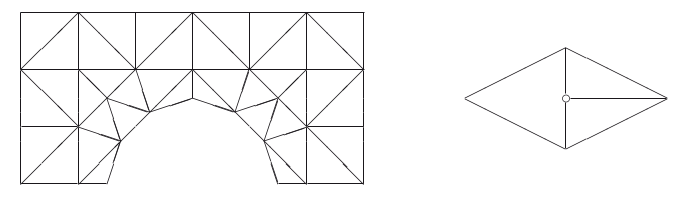
\includegraphics[width=0.8\textwidth]{triangulierung.png} \\
	Abbildung aus \cite{braess2013finite} Seite 58
\end{figure}
Wir werden außerdem im Laufe der Thesis dazu übergehen, ähnlich wie bereits im Abschnitt über die Multilevel Monte Carlo Methode auch bei Zerlegungen von 'Leveln' zu sprechen. Dabei betrachten wir stets eine uniforme Familie zulässiger Zerlegungen $ \{\mathcal{T}_h\}_{h \in \mathcal{H}} $ und fordern dabei, dass die Indexmenge $ \mathcal{H} $ eine ganz bestimmte Form hat. Genauer soll \[ \mathcal{H} = \{ h_0 , h_1 \coloneqq \frac{h_0}{2},h_2 \coloneqq \frac{h_1}{2} = \frac{h_0}{4}, \dots \}  \text{ für ein }  h_0 > 0  \] gelten. Insbesondere gelte also $ \overline{\mathcal{H}} \ni 0 $. Sprechen wir dann von Level $ i $ meinen wir damit die Zerlegung $\mathcal{T}_{h_i} \in \{\mathcal{T}_h\}$.
Zudem führen wir für alle Zerlegungen folgende Bezeichnungen ein:
\begin{itemize}
	\item ein $ K \in \mathcal{T} $ nennen wir Zelle
%	\item $ \mathcal{D}_h \coloneqq \bigcup_{K \in \mathcal{T}} K $ sei die Menge der Zellen
	\item ein $ z \in \mathcal{V}_K \coloneqq \{ z_{K,0} , z_{K,1} , z_{K,2}, z_{K,3}\} \subset \R^2 $ nennen wir Knoten und $\mathcal{V}_K$ die Menge der Knoten von K
	\item $ \mathcal{V}_{\mathcal{T}} \coloneqq \bigcup_{K \in \mathcal{T}} \mathcal{V}_K $ sei die Menge aller Knoten
	\item $\mathcal{F}  \coloneqq (\{ \partial K_1 \cap \partial K_2 : K_1,K_2 \in \mathcal{T} \} \cup \{ \partial K_1 \cap \partial \mathcal{D} : K_1 \in \mathcal{T} \}) \setminus \{\emptyset\} $ sei die Menge aller Seiten
	\item $ \mathcal{F}_K \coloneqq (\{ \partial K \cap \partial K' : K' \in \mathcal{T} \} \cup \{ \partial K \cap \partial \mathcal{D} \}) \setminus \{ \emptyset \} $ sei die Menge aller Seiten von K 
	\item $ \partial \mathcal{D}_h \coloneqq \bigcup_{F \in \mathcal{F}} F $ sei der Rand von $ \mathcal{D}_h $.
\end{itemize}

\subsubsection{Schwache Formulierung}
Betrachten wir also die deterministische Version des Potentialströmungsproblem:
\[ \text{Bestimme } u:\overline{\mathcal{D}} \to \R \text{ und } q: \overline{\mathcal{D}} \to \R^2 \text{ mit } \newline \]
\[\setlength\arraycolsep{1pt}
\text{(PS)}\begin{cases} 
\begin{array}{rlcr}
\dive q     &= 0                 &\text{ ,} \text{in } \mathcal{D} &(1)\\
q           &= - \kappa \nabla u &\text{ ,} \text{in }\mathcal{D} &(2)\\
u           &= u_D               &\text{ ,} \text{auf } \Gamma_D \\
-q \cdot n  &= g_N               &\text{ ,} \text{auf } \Gamma_N 
\end{array}
\end{cases} 
\]
Satz \ref{testfunktionen} sagt uns , dass wir in obiger Formulierung Gleichung (1) mit Testfunktionen $\phi \in H^1(\mathcal{D})$ und Gleichung (2) mit Testfunktionen $\psi \in H^1(\dive,\mathcal{D})$ multiplizieren und anschließend über $\mathcal{D}$ integrieren können und so eine äquivalente schwache Formulierung herleiten:
\begin{align*}
	\int_{\mathcal{D}} \dive(q) \phi \dx &= 0 \text{ für alle Testfunktionen } \phi : \mathcal{D} \to \R \\
	\int_{\mathcal{D}} (q + \kappa \nabla u) \cdot \psi \dx &= 0 \text{ für alle Testfunktionen } \psi : \mathcal{D} \to \R^2
\end{align*}
Da $\kappa$ weiter symmetrisch positiv definit ist, lässt sich letztere Gleichung zu 
\begin{align*}
	&\int_{\mathcal{D}} \kappa^{-1} (q + \kappa \nabla u) \cdot \psi \dx = 0 \\
	\Leftrightarrow \qquad &\int_{\mathcal{D}} \nabla u \cdot \psi \dx = - \int_{\mathcal{D}} (\kappa^{-1}q)\cdot \psi \dx \qquad (\star) 
\end{align*}
umformen. Außerdem wollen wir nun noch die Dirichlet-Randbedingungen $u = u_D \text{ auf } \Gamma_{\text{D}}$ einfließen lassen. Dazu verwenden wir den Satz von Gauß:


\[ \int_{\partial\Omega} (u\psi) \cdot n \da \stackrel{\text{Gauß}}{=} 
 \int_{\Omega} \dive(u\psi) \dx = \int_{\Omega} \nabla u \cdot \psi \dx + \int_{\Omega} u \dive(\psi) \dx \quad (\psi:\Omega \to \R^2) \]
Wählen wir nun unseren Ansatzraum so, dass  für die Funktion $ \psi$ gilt $ \psi \cdot n = 0 \text{ auf } \Gamma_N $. Damit folgt
\begin{align*}
\int_{\Gamma_D} (u_D\psi) \cdot n \da \overset{\psi \cdot n|_{\Gamma_N} = 0}{\underset{u |_{\Gamma_D} = u_D} {=}} \int_{\partial\Omega} (u\psi) \cdot n \da = \underbrace{\int_{\Omega} \nabla u \cdot \psi \dx}_{\stackrel{(\star)}{=}- \int_{\Omega} (\kappa^{-1} q) \cdot \psi \dx } + \int_{\Omega} u \dive(\psi) \dx.
\end{align*}
Die Neumann-Randbedingung $ (\kappa\nabla u) \cdot n = g_N \text{ auf } \Gamma_N $ wird durch die Wahl des Lösungsraumes erfüllt.


Wir erhalten so folgende schwache Formulierung:
\label{sPS}
\begin{align*}
&\text{Bestimme } (q,u) \text{ mit } q\cdot n = -g_N \text{ auf } \Gamma_N \text{ und}\\
&\text{(sPS)}\begin{cases}
\begin{array}{llll}
\int_{\mathcal{D}} \kappa^{-1} q \cdot \psi \dx \, - \mkern-15mu &\int_{\mathcal{D}} u \, \dive(\psi) \dx &= - \int_{\Gamma_D} (u_D \psi) \cdot n \da\\
&\int_{\mathcal{D}} \dive(q) \, \phi \dx &= 0
\end{array}
\end{cases}	\\
&\text{ für alle } (\psi, \phi) \text{ in einem geeigneten Testraum mit } \psi \cdot n = 0 \text{ auf } \Gamma_N 
\end{align*}

\subsubsection{Diskretisierung}
Sei $\mathcal{T}  $ eine zulässige Zerlegung von $ \mathcal{D} $ und alle Bezeichnungen wie oben.
Dabei sei im Weiteren $ N \coloneqq \abs{\mathcal{F}} $ die Anzahl der Seiten und $M = \abs{\mathcal{T}}$ die Anzahl der Zellen.
Wir nummerieren zunächst die Zellen und die Seiten durch:
\begin{align*}
	\mathcal{F} &= \{ F_1,\dots,F_{N}\} \qquad \text{globale Seitennummerierung} \\
	\mathcal{T} &=  \{ K_1,\dots,K_{M}\} \qquad \text{globale Zellennummerierung}
\end{align*}
Als Nächstes soll es nun Ziel sein, eine Lösung der im letzten Abschnitt erklärten schwachen Formulierung in einem endlich dimensionalen Finite Elemente Ansatzraum zu bestimmen. Um aber hierfür genau diese Räume definieren zu können, benötigen wir zuerst sogenannte Basisfunktionen, genauer die Seiten- und die Zellenbasis.\\

 \begin{Definition}(Seiten- und Zellenbasis) 
	\begin{enumerate}[label=(\alph*)]
		\item $ \{ \psi_i \}_{i=1}^{N} $ heißt Seitenbasis und ist definiert durch
			\begin{align*}
					\forall i,j \in \{1, \dots , N \} : \int_{F_j} \psi_i \cdot n^K \da = \pm \delta_{i,j} \text{ und }  \psi_i|_K \in \mathbb{P}_1(K,\R^2) \cap C(\overline{\mathcal{D}}) \ (K \in \mathcal{T}) 
			\end{align*} 
		\item $ \{ \mu_i \}_{i=1}^{M} $ heißt Zellenbasis und ist gegeben durch
			\begin{align*}
				\forall i \in \{1, \dots , M \} : \mu_i \coloneqq  \mathds{1}_{K_i}.
			\end{align*}
	\end{enumerate}
\end{Definition} 

Anschließend können wir mithilfe dieser Basisfunktionen die Testräume bzw. Finite Elemente Räume definieren:
\begin{Definition}(Ansatzräume)
	\begin{enumerate}[label=(\alph*)]
		\item $ W_h \coloneqq \spann \{ \psi_1,\dots,\psi_{N}\}$ (Seitenansatzraum/ Raum für $ \psi $ und $ q_h $)
		\item $ W_h(g) \coloneqq \{ \psi_h \in W_h:  \int_F \psi_h \cdot n \da = \int_F g \da \; \text{ für alle } F \subseteq \Gamma_{\text{N}})  \}$
		\item $ \mathcal{Q}_h \coloneqq \spann \{ \mu_1, \dots, \mu_{M} \} $ (Zellenansatzraum/ Raum für $\phi $ und $ u_h $)
	\end{enumerate}
\end{Definition}

%\begin{Bemerkung}
%	
%	\[	\forall K \in \mathcal{K}:\psi_i|_K \in \mathbb{P}_1(K,\R^2) \text{ und } \mu_m|_K \in \mathbb{P}_0(K,\R) \]
%	Also
%	\begin{align*}	
%	W_h &\subseteq \prod_{K \in \mathcal{K}} \mathbb{P}_1(K,\R^2) &&\text{(Menge der zellenweisen linearen Funktionen) und }\\
%	Q_h &\subseteq \prod_{K \in \mathcal{K}} \mathbb{P}_0(K,\R) &&\text{(Menge der zellenweisen konstanten Funktionen)}. 
%	\end{align*}	
%\end{Bemerkung}

Zusammen mit der schwachen Formulierung \eqref{sPS} erhalten wir so das nun diskretisierte Problem:
\begin{align*}
&\text{Bestimme } (q_h,u_h) \in W_h(-g_N) \times \mathcal{Q}_h \text{ mit}\\
&\begin{cases}
\begin{array}{llll}
\int_{\Omega} \kappa^{-1} q_h \cdot \psi_h \dx \, - \mkern-15mu &\int_{\Omega} u_h \, \dive(\psi_h) \dx &= - \int_{\Gamma_D} (u_D \psi_h) \cdot n \da\\
&\int_{\Omega} \dive(q_h) \, \phi_h \dx &= 0
\end{array}
\end{cases}	\\
&\text{ für alle } (\psi_h, \phi_h) \in W_h(0) \times \mathcal{Q}_h
\end{align*} 




\subsection{Formulierung als LGS}
%Es seien wie bisher Seiten, Seitenbasis, Zellen und Zellenbasis global nummeriert 
%\begin{align*}
%&N \coloneqq \abs{\mathcal{F}} &&\mathcal{F} = \{F_1, \dots , F_{N} \}  \\
%&&&W_h =\{\psi_1, \dots , \psi_N\}\\
%&M \coloneqq \abs{\mathcal{K}} &&\mathcal{K} = \{K_1, \dots , K_{M} \}  \\
%&&&Q_h = \{\mu_1 , \dots , \mu_M  \}.
%\end{align*}

Wir können nun damit beginnen, das so entstandene endlich dimensionale Problem in ein Lineares Gleichungs System umzuformulieren. Dazu definieren wir:
	\begin{align*}
	&\underline{A} \in \R^{N \times N} \text{ mit } \underline{A}[n,k] \coloneqq \int_{\Omega} \kappa^{-1} \psi_n \cdot \psi_k \dx \\
	&\underline{B} \in \R^{M \times N} \text{ mit } \underline{B}[m,k] \coloneqq - \int_{\Omega} \mu_m \dive(\psi_k) \dx \\
	&\underline{b} \in \R^N \text{ mit } \underline{b}[k] \coloneqq - \int_{\Gamma_D} u_D \psi_k \cdot n \da
	\end{align*}
	und (für die Randbedingungen)
	\begin{align*}
	\underline{W}(g) \coloneqq \left\{ \underline{q} \in \R^N : \underline{q}[k] = \int_{F_k} g  \da \ (\text{für } k \text{ mit } F_k \subseteq \Gamma_N) \right\} 
	\end{align*}


Unser zu lösendes Problem lässt sich so mit $ q_h = \sum_{n=1}^{N} \underline{q}[n] \psi_n $ und $ u_h = \sum_{m=1}^{M} \underline{u}[m] \mu_m $ umformen zu 
\begin{align*}
\text{Bestimme} (\underline{q},\underline{u}) \in \underline{W}(-g_N)\times \R^{M} \text{ mit }\\
\begin{cases}
\underline{A} \underline{q} + \underline{B}^T \underline{u} &= \underline{b} \\
\underline{B} \underline{q} &= 0
\end{cases}
\end{align*}
oder anders geschrieben 
\begin{align*}
\text{Bestimme} (\underline{q},\underline{u}) \in \underline{W}(-g_N)\times \R^{M} \text{ mit }\\
\begin{cases}
\begin{pmatrix}
\underline{A} &\underline{B}^T\\
\underline{B} &0
\end{pmatrix}
\begin{pmatrix}
\underline{q} \\
\underline{u} 
\end{pmatrix}
=
\begin{pmatrix}
\underline{b}\\
0
\end{pmatrix}.
\end{cases}
\end{align*}

Wir haben so eine diskrete gemischte Formulierung des Potentialströmungsproblems hergeleitet und können mit dieser aus gegebenen Rand- und Anfangswerten ein Flussvektorfeld $q$ erzeugen, welches der obigen Differentialgleichung genügt.
Es handelt sich hierbei um das gemischte Finite Elemente Verfahren. In M++ selbst lösen wir das Potentialströmungsproblem durch eine Abwandlung dieses Verfahrens. Wir diskretisieren dazu eine äquivalente Formulierung von (sPS) und erhalten so mit dem hybriden Finite Elemente Verfahren die gleichen Ergebnisse, die auch der vorgestellte gemischte Ansatz liefern würde, bei besserer Effizienz und guter Parallelisierbarkeit. Da das Potentialströumgsproblem in dieser Thesis primär dazu genutzt werden soll, das Vektorfeld $q$ zu bestimmen, soll uns aus theoretischer Sicht aber obige Formulierung genügen und wir verweisen hinsichtlich der Lösung mit hybriden gemischten Finiten Elementen, neben einem kleinen, Überblick verschaffendem Abschnitt im Appendix \ref{Referenzzelle&Hyb}, auf die Literatur, wie etwa \cite{brezzi2012mixed} oder  \cite{roberts1991mixed}.












%%%%%%%%%%%%%%%%%%%%%%%%%%%%%%%%%
\newpage  % neuer Abschnitt auf neue Seite, kann auch entfallen
%%%%%%%%%%%%%%%%%%%%%%%%%%%%%%%%%
\subsection{Numerische Lösung des Transportproblem}
% !TeX root = bachelorarbeit.tex
 \label{DG}
In diesem Abchnitt soll nun, nachdem wir $q(\omega,\cdot)$ als Finite-Elemente-Lösung des Potentialströmungsproblems erhalten haben, die numerische Lösung des linearen Transportproblems behandelt werden:
\begin{align*}
	&\text{Für } \omega \in \Omega \text{ und }q(\omega,\cdot): \overline{\mathcal{D}} \to \R^2 \text{, bestimme }\rho(\omega,\cdot): \overline{\mathcal{D}} \times \mathbb{T} \to \R_{\geq 0} \text{ mit} \\
	&\text{(pTP)} 
	\begin{cases}
	\begin{array}{rlll}
	\partial_t \rho (\omega, x, t) + \dive(\rho(\omega,x,t)q(\omega,x)) &= 0 &\text{, für } (x,t) \in \mathcal{D} \times (0,T] \\
	\rho(\omega,x,t) &= \rho_{\text{in}}(x,t) &\text{, für } (x,t) \in \Gamma_{\text{in}} \times \mathbb{T} \\
	\rho(\omega,x,0)  &= \rho_0(x) &\text{, für } x \in  \mathcal{D}
	\end{array}
	\end{cases} \\
\end{align*}
Insbesondere wollen wir an dieser Stelle wieder $\omega \in \Omega$ festhalten und betrachten deshalb zunächst nur das deterministische Problem wie in \ref{det_prob}:
\[ 
\text{Bestimme } \rho: \overline{\mathcal{D}} \times \mathbb{T} \to \R_{\geq 0} \text{, sodass} \newline \]
\[\setlength\arraycolsep{1pt}
\text{(dTP)}\begin{cases} 
\begin{array}{rlll}
\partial_t \rho(x,t) + \dive(\rho(x,t) q(x)) &= 0 &\text{ ,in } &\mathcal{D} \times (0,T)\\
\rho(x,t) &= \rho_{\text{in}}(x,t) &\text{ ,auf } &\Gamma_{\text{in}} \times (0,T)\\
\rho(x,0) &= \rho_0(x) &\text{ ,auf } &\mathcal{D} \\
\end{array}
\end{cases} \\
\]
 Wir greifen dabei auf ein sogenanntes discontinuous Galerkin Verfahren zurück, welches für diese Problemklasse bereits an anderen Stellen (z.B. in \cite{cockburn1998runge}) erprobt wurde. Ursprünglich geht das Discontinuous Galerkin Verfahren auf Reed und Hill \cite{reed1973triangular} zurück. Einen guten (wenn auch mittlerweile etwas in die Jahre gekommenen) Überblick über die Anwendung von discontinuous Galerkin Verfahren bietet \cite{cockburn2000development}.
Grundätzlich handelt es sich beim discontinuous Galerkin Verfahren ebenfalls um einen FEM Ansatz, der zwar Ähnlichkeiten zum Finite Elemente Verfahren aufweist, welches wir im letzten Abschnitt gesehen hatten, aber auch einige bedeutende Unterschiede besitzt, auf welche wir im Folgenden besonders eingehen wollen. 
%So werden wir wieder eine schwache Formulierung des analytischen Problems herleiten und uns dann im Rahmen des diskretisierung erneut auf endlich dimensionale Räume zurückziehen.
Anders als zuvor das Potentialströmungsproblem ist die lineare Transportgleichung  nämlich sowohl orts- als auch zeitabhängig. Daher werden wir
%, nachdem wieder zuerst eine schwache Formulierung eingeführt wird,
  die lineare Transportgleichung zunächst im Ort diskretisieren. Wir erhalten so eine Semidiskretisierung, welche wir anschließend mit einem Zeitintegrator, wie beispielsweise der impliziten Mittelpunktsregel, in eine Volldiskretisierung überführen.
 

%\subsubsection{Schwache Formulierung}
%Wie im letzten Abschnitt führen wir nun einen schwachen Lösungsbegriff ein. Sei dazu $ \phi : \mathcal{D} \times \mathbb{T} \to \R $ eine beliebige Testfunktion, etwa aus  $W_0^{1,2}(\mathcal{D} \times \mathbb{T}) $, für die $ \phi(\cdot,T) = 0 $ gelte. 
%Wir beginnen mit der differentialgleichung $ \partial_t \rho(x,t) + \dive(\rho(x,t) q(x)) = 0  $, multiplizieren zunächst mit der Testfunktion $ \phi $ und integrieren anschließend über den Raum-Zeitzylinder $ \mathcal{D} \times \mathbb{T} $:
%\begin{align*}
%	\int_{\mathcal{D} \times \mathbb{T}} \big(\partial_t \rho(x,t) &+ \dive(\rho(x,t) q(x) ) \big) \phi(x,t) \; \mathrm{d} (x,t) =  \\
%	&\underbrace{\int_{\mathcal{D} \times \mathbb{T}}  \partial_t \rho(x,t) \phi(x,t) \; \mathrm{d} (x,t)}_{(1)} +\underbrace{\int_{\mathcal{D} \times \mathbb{T}}  
%    \dive(\rho(x,t) q(x) ) \phi(x,t)\; \mathrm{d} (x,t)}_{(2)}
%\end{align*}
%Betrachten wir nun zunächst Integral (1), so folgt mit partieller Integration:
%\begin{align*}
%	\int_{\mathcal{D} \times \mathbb{T}}  \partial_t \rho(x,t) &\phi(x,t) \; \mathrm{d} (x,t) = \int_{\mathcal{D}} \int_{\mathbb{T}} \partial_t \rho(x,t) \phi(x,t) \dt \dx \\&= \int_{\mathcal{D}} \big( - \int_{\mathbb{T}} \rho(x,t) \partial_t \phi(x,t) \dt + \big[ \rho(x,t) \phi(x,t) \big]_0^T  \big) \dx \\
%	&= - \int_{\mathcal{D} \times \mathbb{T}} \rho(x,t) \partial_t \phi(x,t) \; \mathrm{d} (x,t) + \int_{\mathcal{D}} \underbrace{\rho(x,T) \phi(x,T)}_{ = 0 } - \underbrace{\rho(x,0)}_{ = \rho_0(x) \text{ auf } \mathcal{D}} \phi(x,0)  \dx\\
%	&= - \int_{\mathcal{D} \times \mathbb{T}} \rho(x,t) \partial_t \phi(x,t) \; \mathrm{d} (x,t) - \int_{\mathcal{D}} \rho_0(x) \phi(x,0) \dx 
%\end{align*}
%Außerdem können wir Integral (2) mit  \ref{n_pI} wie folgt ausdrücken:
%\begin{align*}
%	\int_{\mathcal{D} \times \mathbb{T}}  
%	\dive(\rho(x,t) &q(x) ) \phi(x,t)\; \mathrm{d} (x,t) = \int_{\mathbb{T}} \int_{\mathcal{D}} \dive(\rho(x,t) q(x) ) \phi(x,t) \dx \dt \\
%	&= \int_{\mathbb{T}} \big( - \int_{\mathcal{D}} \rho(x,t) q(x) \nabla \phi(x,t) \dx + \int_{\partial \mathcal{D}} \rho(x,t) q(x) \cdot n \ \phi(x,t) \da \big)  \dt \\
%	&= - \int_{\mathcal{D} \times \mathbb{T}} \rho(x,t) q(x) \nabla \phi(x,t)) \; \mathrm{d} (x,t) + \int_{\mathbb{T}} \int_{\partial \mathcal{D}} \rho(x,t) q(x) \cdot n \phi(x,t) \da \dt 
%\end{align*}
%Mit $ \partial \mathcal{D} = \Gamma_{\text{in}} \dot{\cup} \Gamma_{\text{out}} $ und 
%$\rho(x,t) = \rho_{\text{in}}(x,t) \text{ für } (x,t) \in \Gamma_{\text{in}} \times (0,T)$ erhalten wir so die folgende Formulierung:
%\begin{definition} 
%$ \rho \in L_1 (\mathcal{D} \times (0,T)) $ heißt schwache Lösung des linearen Transportproblems, falls es für ein gegebenes $ q : \overline{\mathcal{D}} \to \R^2 $ folgende Bedingungen erfüllt:
%\begin{align*}
%\text{(swTP)}
%\begin{cases}
%\begin{array}{rlll}
%\displaystyle
%\int_{\mathcal{D}} \rho_0 \phi(0) \dx = \mkern-16mu &- \displaystyle \int_{0}^{T} \int_{\mathcal{D}} \rho (\partial_t \phi + q \nabla \phi ) \dx \dt \\
%&+\displaystyle\int_{0}^{T}  \int_{\Gamma_{\text{in}}} \rho_{\text{in}} q \cdot n \phi \da  \dt \\
%&+\displaystyle\int_{0}^{T}  \int_{\Gamma_{\text{out}}} \rho q \cdot n \phi \da  \dt
%\end{array}
%\end{cases}	
%\end{align*}
%für alle Testfunktionen $ \phi: \mathcal{D} \times (0,T) \to \R $ mit $ \phi(\cdot,T) = 0 $ auf $ \mathcal{D}  $ und $ \phi|_{\Gamma_{\text{out}}} = 0 $.
%\end{definition}
%dabei ist $  \Gamma_{\text{out}} \coloneqq  \{ z \in \partial \mathcal{D}: q(z)\cdot n(z) > 0 \}$ 
%und $  \Gamma_{\text{in}} \coloneqq  \{ z \in \partial \mathcal{D}: q(z)\cdot n(z) \leq 0 \} $. \\
%Obige Herleitung zeigt zusammen mit \ref{testfunktionen} insbesondere die Gültigkeit des folgenden Zusammenhangs zwischen klassischen Lösungen der linearen Transportgleichung und schwachen Lösungen von (swTP):
%
%\begin{Lemma}(Zusammenhang der Lösungsbegriffe)
%	\begin{enumerate}
%		\item Ist $ \rho $ eine klassische Lösung, so ist $ \rho $ auch eine schwache Lösung.
%		\item Ist $ \rho \in C^2(\mathcal{D} \times \mathbb{T} , \R )$ und eine schwache Lösung, so ist $ \rho $ auch eine klassische Lösung. 
%	\end{enumerate}
%\end{Lemma}
\subsubsection{Diskretisierung}
\label{Diskretisierung}
Wie bereits weiter oben beschrieben, werden wir im Folgenden zunächst den Raum diskretisieren und anschließend die so entstandene Semidiskretisierung in eine Volldiskretisierung auflösen. Insgesamt wollen wir das discontinuous Galerkin Verfahren mit einem Zeitintegrator, wie der impliziten Mittelpunktsregel oder einem klassischen Runge-Kutta-Verfahren nutzen. Zunächst führen wir die analytische Flussfunktion ein. 
\begin{Definition}(Flussfunkion) \\
	\label{Flussfunktion}
	Zu einem gegebenen Flussvektorfeld $ q : \mathcal{D} \to \R^2 $ ist die Flussfunktion $ \Upsilon$ definiert als:\\
	\begin{align*}
		 \Upsilon : \text{Abb}(\mathcal{D}\times\mathbb{T},\R) &\to \text{Abb}(\mathcal{D}\times\mathbb{T},\R^2) \\
		 \rho &\mapsto \rho q
	\end{align*}
\end{Definition}
$\newline$
Für eine klassische Lösung $ \rho  $ von (dTP) gilt dann insbesondere $ \partial_t \rho = - \dive (\Upsilon(\rho)) $ auf $ \mathcal{D} \times (0,T] $.	\\
Halten wir also zunächst $ t \in \mathbb{T} $ und leiten so die Semidiskretisierung her.\\
Sei nun $ \mathcal{T} $ eine zulässige Triangulierung von $ \mathcal{D} $ aus Dreiecken wie in \ref{num_pot} und  $ (\cdot , \cdot)_A $ das $ L^2(A)-$Skalarprodukt.
Wir wählen als Lösungs-/Testraum $\mathcal{Q}_h = \prod_{K \in \mathcal{T}} \mathbb{P}_p(K,\R) $ für ein festes $p \geq 1 $. Anders als zuvor fordern wir für unsere Lösungs- und Testfunktionen diesmal aber \underline{nicht} die Stetigkeit auf $\mathcal{D}$. Da so $\mathcal{Q}_h$ nicht im betrachteten analytischen Lösungs- und Testraum liegt, etwa  $\mathcal{Q}_h \nsubseteq H^1(\mathcal{D})$, nennt man $\mathcal{Q}_h$ auch einen nicht-konformen Ansatzraum.
Außerdem lässt sich im Allgemeinen auch die später bestimmte Lösung $ \rho_h \in \mathcal{Q}_h $ (definiert auf $\mathcal{D}_h = \bigcup_{K \in \mathcal{T}} K$ ) nicht stetig auf $ \mathcal{D} $ fortsetzen, denn für eine beliebige innere Kante $ F $ kann der Grenzwert von $ \rho_h $ auf den anliegenden Zellen $ K,K' $ ($ \overline{F} = \partial K \cap \partial K' $) unterschiedlich sein. \\
Trotzdem müssen wir auch auf den inneren Kanten $ \mathcal{F}^0 \subset \mathcal{F} $ festlegen, welcher Grenzwert in einem solchen Falle gewählt wird. \\
Dazu führen wir als Pendant zur analytischen Flussfunktion (vgl. \ref{Flussfunktion})
auch eine numerische Flussfunktion ein. Grundsätzlich kommen mehrere solche Flussfunktionen in Frage, welche direkten Einfluss auf Eigenschaften des entstehenden Verfahrens besitzen. Wir entscheiden uns an dieser Stelle für den weit verbreiteten 
sogenannten upwind flux:
\begin{Definition}(upwind flux)\\
	Sei $K \in \mathcal{T}$ eine beliebige Zelle und $ F \in \mathcal{F}_K$ eine Kante von $K$. Dann ist
	\begin{align*}
		\Upsilon^{\star} : \text{Abb}(\mathcal{D}\times\mathbb{T},\R) &\to \text{Abb}(\mathcal{D}\times\mathbb{T},\R^2) \\
		\rho_h &\mapsto 
		\begin{cases}
			\Upsilon(\rho_h|_K) , \ \text{ für } q\cdot n_F^K \geq 0 \\  
			\Upsilon(\rho_h|_{K'}) ,\text{ für } q\cdot n_F^K < 0 \text{ und } \overline{F} = \partial K \cap \partial K'
		\end{cases}
	\end{align*}
\end{Definition}
Sei nun also $ \rho $ klassische Lösung von (dTP) mit $ \partial_t \rho = -\dive(\Upsilon(\rho)) $ auf $ \mathcal{D} $. Dann gilt nach Satz von Gauß:
\begin{align}
		\label{gaus1}
		\int_{\partial \mathcal{D}} \rho q \cdot n \phi \da  =\int_{\partial \mathcal{D}} \Upsilon(\rho) \cdot n \phi \da = \int_{\mathcal{D}} \dive (\Upsilon(\rho)\phi) \dx
\end{align}
Das Integral über den Rand von $ \mathcal{D} $ können wir nach der folgenden kleinen Vorüberlegung auch als Integral über alle Kanten der gewählten Zerlegung $ \mathcal{T} $ ausdrücken: \\
Es gilt nämlich für alle inneren Kanten, also solche Kanten $ F $, für die zwei Zellen $ K $ und $ K' $ existieren, sodass $ \overline{F} = K \cap K' $ ist, dass $ \int_F \Upsilon^{\star}(\rho) \cdot n^K \phi \da = - \int_F \Upsilon^{\star}(\rho) \cdot n^{K'} \phi \da $ stets erhalten ist. \\
Summieren wir also zunächst über alle Zellen, summieren anschließend die Integrale über alle Kanten und ersetzen dabei den analytischen durch den numerischen Fluss, erhalten wir gerade wieder obiges Randintegral. Es gilt also:
\begin{align*}
	\sum_{K\in \mathcal{T}} \sum_{F \in \mathcal{F}_K} \int_F \Upsilon^{\star}(\rho) \cdot n^K \phi \da = \int_{\partial \mathcal{D}} \Upsilon(\rho) \cdot n \phi \da \stackrel{\text{\ref{gaus1}}}{=} \int_{\mathcal{D}} \dive (\Upsilon(\rho)\phi) \dx
\end{align*}
Nach der Produktregel der Divergenz lässt sich das letzte Integral auswerten zu:
\begin{align*}
	 \int_{\mathcal{D}} \dive (\Upsilon(\rho)\phi) \dx = \int_{\mathcal{D}} \phi \dive(\Upsilon(\rho)) + \Upsilon(\rho) \cdot \nabla \phi \dx \stackrel{\text{ Vor.}}{=} - \int_{\mathcal{D}} \partial_t \rho \phi \dx + \int_{\mathcal{D}} \Upsilon(\rho) \cdot \nabla \phi \dx
\end{align*}
Durch Umstellen und das Zusammenfassen der obigen Resultate erhalten wir so: 
\begin{align*}
	\sum_{K \in \mathcal{T}} \int_K \partial_t \rho  \phi \dx = \sum_{K \in \mathcal{T}} \int_K \Upsilon(\rho ) \cdot \nabla \phi \dx - 	\sum_{K\in \mathcal{T}} \sum_{F \in \mathcal{F}_K} \int_F \Upsilon^{\star}(\rho) \cdot n^K \phi \da
\end{align*}
Dabei wurde zusätzlich ausgenutzt, dass es sich bei den Kanten um Nullmengen handelt und wir so das Integral über $ \mathcal{D} $ als Summe der Integrale über alle Zellen auffassen können. Nutzen wir nun noch aus, dass für den Fluss  $\rho(x,t) = \rho_{\text{in}}(x,t)$ für $ x \in \Gamma_{\text{in}} $ gilt, kommen wir so auf 
\begin{align}
	\label{fastfertigsemi}
	\sum_{K \in \mathcal{T}} \int_K \partial_t \rho  \phi \dx = \sum_{K \in \mathcal{T}} \int_K \Upsilon(\rho ) \cdot \nabla \phi \dx - 	\sum_{K\in \mathcal{T}} \left( \sum_{\substack{F \in \mathcal{F}_K \\ F \not\subseteq \Gamma_{\text{in}}}} \int_F \Upsilon^{\star}(\rho) \cdot n^K \phi \da - \sum_{\substack{F \in \mathcal{F}_K \\ F \subseteq \Gamma_{\text{in}}}} \rho_{\text{in}} q \cdot n^K \phi \da \right)
\end{align}
Sei nun $ \mathcal{T} = \{ K_1,\dots , K_N\} , N \coloneqq |\mathcal{T}| $. Die Semidiskretisierung ist motiviert durch (\ref{fastfertigsemi}) und lautet: Bestimme  $\rho_h \in \mathcal{Q}_h$, sodass für alle $ \phi_h \in \mathcal{Q}_h $ gilt:
\begin{align}
	\label{Semidiskretisierung}
	\sum_{i=1}^N (\partial_t \rho_h, \phi_h)_{K_i} &= \sum_{i=1}^{N} \big( (\Upsilon(\rho_h), \nabla \phi_h)_{K_i} - \sum_{\substack{F \in \mathcal{F}_K \\ F \not \subseteq \Gamma_{\text{in}}}}(\Upsilon^{\star}(\rho_h)\cdot n^K,\phi_h)_{F} - (\rho_{\text{in}}q \cdot n^K,\phi_h)_{\partial K_i \cap \Gamma_{\text{in}}} \big)
\end{align}


Durch Einsetzen der Zellenbasis $ \{\mu_i\}_{i=1}^N \subset \mathcal{Q}_h $  und mit $ \supp(\mu_i) \subseteq \overline{K_i} (\ i \in \{1, \dots , N\})$ ergibt sich für alle $\ i \in \{1, \dots , N\}$ : \\
TODOOOOOOOOOOOOOOOO überarbeiten
\begin{align*} 
\left(\partial_t \rho_h, \mu_i  \right)_{K_i}  &= \bigg( \underbrace{(\Upsilon(\rho_h), \nabla\mu_i)_{K_i}}_{=0 \text{, da } \nabla \mu_i = 0} - \sum_{\substack{F \in \mathcal{F}_{K_i} \\ F \not\subseteq \Gamma_{\text{in}}}} \left(\Upsilon^*(\rho_h) \cdot n^{K_i}, \mu_i \right)_{F} - \left(\rho_{\text{in}} q \cdot n^{K_i}, \mu_i \right)_{\partial K_i \cap \Gamma_{\text{in}}} \bigg) \\
\end{align*}
Wir erhalten so folgende Darstellung:
%\begin{align*}
%\left(\partial_t \rho_h, \mu_i  \right)_{K_i} = \bigg( - \sum_{\substack{F \in \mathcal{F}_{K_i}, F \not\subseteq \Gamma_{\text{in}}\\ F \text{ mit }q \cdot n^K_{|F} > 0} } \left(\underbrace{\Upsilon^*(\rho_h)}_{= \rho_{h|K}\, q} \cdot n^{K_i}, \mu_i \right)_{F} - \sum_{\substack{F \in \mathcal{F}_{K_i}, F \not\subseteq \Gamma_{\text{in}}\\ F \text{ mit }q \cdot n^K_{|F} < 0} } \left(\underbrace{\Upsilon^*(\rho_h)}_{= \rho_{h|K'} \, q} \cdot n^{K_i}, \mu_i \right)_{F}\\
% - \left(\rho_{\text{in}} q \cdot n^{K_i}, \mu_i \right)_{\partial K_i \cap \Gamma_{\text{in}}} \bigg)
%\end{align*} 

\begin{align}
\label{DarstellungvorLGS}
\underbrace{\left(\partial_t \rho_h, \mu_i  \right)_{K_i}}_{(\ref{DarstellungvorLGS}.1)} = 
\underbrace{-  \sum_{F \in \mathcal{F}_{K_i} , F \not \subseteq \Gamma_{\text{in}}}\left(\Upsilon^{\star}(\rho_h)\cdot n^{K_i},\mu_i\big)_F \right)}_{(\ref{DarstellungvorLGS}.2)} \underbrace{- \left(\rho_{\text{in}}q\cdot n^{K_i},\mu_i \right)_{\partial K_i \cap \Gamma_{\text{in}}}}_{(\ref{DarstellungvorLGS}.3)}
\end{align}

Zusammen mit der Basisdarstellung von $ \rho_h $ in $\{\mu_i  \}_{i=1}^N$, $ \rho_h = \sum_{i=1}^{N} 
\underline{\rho}[i] \; \mu_i$, und \\
$ \Upsilon^{\star}(\rho_h) = 
\begin{cases} 
\rho_h|_K \ ,\text{falls } q\cdot n^K|_F \geq 0\\
\rho_{h}|_{K'} \ , \text{falls } q\cdot n^K|_F < 0
\end{cases} $ können wir \ref{DarstellungvorLGS} in eine gewöhnliche Differentialgleichung erster Ordnung umformulieren. 
Dazu klammern wir jeweils $ \underline{\rho} $ aus und definieren 
\begin{align*}
&\text{mithilfe von (\ref{DarstellungvorLGS}.1) die Massenmatrix } \underline{M}\in \R^{N \times N} \\  &\qquad \qquad \underline{M}[K,K'] \coloneqq \begin{dcases}
\int_K \abs{\mu_K}^2 \dx & \text{, für } K = K' \\
0 &\text{, sonst}
\end{dcases} \\
&\text{mit (\ref{DarstellungvorLGS}.2) die Flussmatrix } \underline{A}\in \R^{N \times N} \\ &\qquad \qquad \underline{A}[K,K'] \coloneqq \begin{dcases}
- \sum_{\substack{F\in \mathcal{F}_K \\ F \text{ mit } q\cdot n^K_{|F} > 0}} \int_F \mu_K^2 q \cdot n^K \da& \text{, für } K = K' \\
- \int_F \mu_K \mu_{K'} q \cdot n^K \da &\text{, für } q \cdot n^K< 0 \text{ und } \overline{F} = \partial K \cap \partial K'\\
0 &\text{, sonst}
\end{dcases} \\
&\text{und mit (\ref{DarstellungvorLGS}.3) den Lastvektor } \underline{b}\in \R^{N} \\ &\qquad \qquad\underline{b}[K] \coloneqq \int_{\partial K \cap \Gamma_{\text{in}}} \rho_{\text{in}} q \cdot n \da
\end{align*}
So ergibt sich die Differentialgleichung
\begin{align*}
\begin{cases}
\underline{M} \partial_t \underline{\rho}(t) = \underline{A} \underline{\rho}(t) + \underline{b}(t) \\
\underline{\rho}(0) = \underline{\rho_0}
\end{cases}\\
\end{align*}
Da dies nun eine gewöhnliche Differentialgleichung ist, können wir die Lösung 
\begin{align}
 \label{semidisklsg}
 \underline{\rho}(t) = \exp(t \underline{M}^{-1} \underline{A}) \left( \underline{\rho_0} + \int_{0}^{t} \exp(-s\underline{M}^{-1} \underline{A}) \underline{b}(s) \ds \right)
\end{align}
explizit angeben.
Es handelt sich hierbei aber immer noch um eine semidiskrete Formulierung. 
Wir wollen deshalb zuletzt noch auf die Herleitung der Zeitintegratoren eingehen. Diese nutzen wir, um unter Verwendung der oben hergeleiteten Semidiskretisierung die numerische Lösung $ \underline{\rho} $ sowohl orts- al auch zeitdiskret zu berechnen. Der Ansatz leitet sich hierbei direkt aus dem Resultat (\ref{semidisklsg}) ab und besteht aus der 
Integration der Differentialgleichung $\underline{M} \partial_t \underline{\rho} = \underline{A} \underline{\rho} + \underline{b}$ über die Zeit $t$ im Intervall $[t_i, t_{i+1}]$.
Dabei ist $t_i = i \delta t$. Hiermit folgt:
\begin{align*}
\underline{M}\underline{\rho}(t_{i+1}) - \underline{M}\underline{\rho}(t_i) = \int_{t_i}^{t_{i+1}}
\underline{M} \partial_t \underline{\rho}(t) dt =\int_{t_i}^{t_{i+1}} \underline{A} \underline{\rho}(t) + \underline{b}(t) dt.
\end{align*}
Mithilfe der Anwendung verschiedener Quadraturformeln lässt sich daraus ein Runge-Kutta Verfahren herleiten. Über die Rechteckformel 
\begin{align*}
\int_{t_i}^{t_{i+1}}\underline{A} \underline{\rho}(t) + \underline{b} dt \approx (t_{i+1}-t_i)( 
\underline{A} \underline{\rho}(t_{i+1}) + \underline{b}(t_{i+1})) = \delta t (\underline{A} \underline{\rho}(t_{i+1}) + \underline{b}(t_{i+1}))
\end{align*}
ergibt sich z.B. das implizite Euler Verfahren
\begin{align*}
\underline{\rho}(t_{i+1}) = \underline{\rho}(t_{i}) + \delta t \underline{M}^{-1}(\underline{A} \underline{\rho}(t_{i+1}) + \underline{b}(t_{i+1})).
\end{align*}
%Weitere Verfahren, die wir verwenden werden, sind zum einen das
%klassische Runge-Kutta Verfahren (der Übersicht wegen für $\underline{b} \equiv 0$)
%\begin{align*}
%\underline{\rho}(t_{i+1}) = \underline{\rho}(t_{i}) +
%\delta t \underline{M}^{-1}\underline{A} (
%\underline{\rho}(t_{i}) +
%\frac{\delta t}{2} \underline{M}^{-1}\underline{A} (
%\underline{\rho}(t_{i}) +
%\frac{\delta t}{3} \underline{M}^{-1}\underline{A} (
%\underline{\rho}(t_{i}) +
%\frac{\delta t}{4} \underline{M}^{-1}\underline{A} 
%\underline{\rho}(t_{i}) )))
%\end{align*}
%und zum anderen die implizite Mittelpunktsregel 
Ein weiteres Verfahren dieser Art, welches wir an dieser Stelle verwenden werden, ist die implizite Mittelpunktsregel (der Übersicht wegen für $\underline{b} \equiv 0$):
\begin{align*}
\underline{\rho}(t_{i+1}) = \underline{\rho}(t_{i}) +
\delta t \underline{M}^{-1} (
\underline{A} 
\frac{1}{2}(\underline{\rho}(t_{i}) +
\underline{\rho}(t_{i+1}) )
+
\frac{1}{2} ( \underline{\rho}(t_{i}) +
\underline{\rho}(t_{i+1}) )).
\end{align*}

Das so entstehenden Gesamtverfahren ist aufgrund der Kombination von Discontinuous Galerkin Verfahren und Runge-Kutta-Zeitintegratoren in der Literatur oft auch unter dem Namen 'Runge–Kutta discontinuous Galerkin Methods' zu finden. Einen schönen Überblick über diese Verfahrensklasse bietet der Artikel \cite{cockburn2001runge}.
Nachdem wir nun das Discontinuous Galerkin Verfahren für die lineare Transportgleichung eingeführt und erklärt haben, sollen nun noch auf einige Eigenschaften des Verfahrens verwiesen werden. Dabei wollen wir uns aber beschränken, einige grundlegende Resultate zu nennen und so eher einen groben Überblick mit Referenzen zur Literatur zu geben. Mehr zur numerischen Analyse des Discontinuous Galerkin Verfahren findet sich zum einen in Standardwerken, wie \cite{ern2004theory}, eine schöne Zusammenstellung bietet aber auch
\cite{Har08b}. \\
Ebenfalls findet sich in \cite{Har08b} eine grundlegende numerische Analyse des Discontinuous Galerkin Verfahrens angewandt auf die stationäre lineare Transportgleichung. Dabei werden unter anderem die Konsistenz, die sogenannte Galerkin-Orthogonalität, sowie die Stabilität und Konvergenz des Verfahrens behandelt.
Mit der numerischen Analyse des Discontinuous Galerkin Verfahrens an sich befassten sich unter anderem LeSaint und Raviart \cite{lesaint1974finite}, Peterson \cite{peterson1991note} und Richter \cite{richter1988optimal}.
Runge-Kutta DG Verfahren für der linearen Transportgleichung ähnliche Problemstellungen betrachteten Cockburn und Shu in einer 5-teiligen Serie von Arbeiten. Besonders zu nennen sind dabei in unserem Kontext \cite{cockburn1989tvb} und \cite{cockburn1990runge}.


\subsection{Eigenschaften des Discontinuous Galerkin Verfahren}
Nachdem wir nun das Discontinuous Galerkin Verfahren für die lineare Transportgleichung eingeführt und erklärt haben, sollen noch einige Eigenschaften des Verfahrens beleuchtet werden. Dabei wollen wir uns aber darauf beschränken, einige grundlegende Resultate zu nennen, und so eher einen groben Überblick mit Referenzen zur Literatur zu geben. Mehr zur numerischen Analyse des Discontinuous Galerkin Verfahren findet sich zum einen in Standardwerken, wie \cite{ern2004theory}, eine schöne Zusammenstellung bietet aber auch \cite{Har08b}.
Ebenfalls findet sich in \cite{Har08b} eine grundlegende numerische Analyse des Discontinuous Galerkin Verfahrens auf die stationäre lineare Transportgleichung.
\subsubsection{Lösungsbegriffe}
	Wie zuvor bereits beim Potentialströmungsproblem können wir auch für das Transportproblem eine sogenannte schwache Formulierung bestimmen. Diese hängt im Fall des Transportproblems eng mit der Semidiskretisierung zusammen und lautet mit $ \partial \mathcal{D} = \Gamma_{\text{in}} \dot{\cup} \Gamma_{\text{out}} $ und 
$\rho(x,t) = \rho_{\text{in}}(x,t) \text{ für } (x,t) \in \Gamma_{\text{in}} \times (0,T)$ :
\begin{Definition} 
	$ \rho \in L_1 (\mathcal{D} \times (0,T)) $ heißt schwache Lösung des linearen Transportproblems, falls es für ein gegebenes $ q : \overline{\mathcal{D}} \to \R^2 $ folgende Bedingungen erfüllt:
	\begin{align*}
	\begin{array}{rllll}
	&\text{(swTP)} \ &B(\rho,\phi) &= \langle b,\phi\rangle \quad \forall \phi \in H^1(\mathcal{D}\times\mathbb{T}) \text{ mit } \phi(\cdot,T) = 0 \text{ und } \phi|_{\Gamma_{\text{out}}} = 0 \\
	&\text{Dabei sind :} & & &\\
	& &B(\rho,\phi) &\coloneqq  \int_{0}^{T} \int_{\mathcal{D}} \rho (\partial_t \phi + q \nabla \phi ) \dx \dt - \int_{\Gamma_{\text{out}}} \rho q \cdot n \phi \da  \dt \\
	& &\langle b,\phi \rangle &\coloneqq \int_{\Gamma_{\text{in}}} \rho_{\text{in}} q \cdot n \phi \da  \dt - \int_{\mathcal{D}} \rho_0 \phi(0) \dx \\
	& & \Gamma_{\text{out}} &\coloneqq  \{ z \in \partial \mathcal{D}: q(z)\cdot n(z) > 0 \} & \\
	& & \Gamma_{\text{in}} &\coloneqq  \{ z \in \partial \mathcal{D}: q(z)\cdot n(z) \leq 0 \} &
	\end{array}\\
	%		\text{(swTP)}
	%		\begin{cases}
	%		\begin{array}{rlll}
	%		\displaystyle
	%		\int_{\mathcal{D}} \rho_0 \phi(0) \dx = \mkern-16mu &- \displaystyle \int_{0}^{T} \int_{\mathcal{D}} \rho (\partial_t \phi + q \nabla \phi ) \dx \dt \\
	%		&+\displaystyle\int_{0}^{T}  \int_{\Gamma_{\text{in}}} \rho_{\text{in}} q \cdot n \phi \da  \dt \\
	%		&+\displaystyle\int_{0}^{T}  \int_{\Gamma_{\text{out}}} \rho q \cdot n \phi \da  \dt
	%		\end{array}
	%		\end{cases}	
	\end{align*}
	%		für alle Testfunktionen $ \phi: \mathcal{D} \times (0,T) \to \R $ mit $ \phi(\cdot,T) = 0 $ auf $ \mathcal{D}  $ und $ \phi|_{\Gamma_{\text{out}}} = 0 $.
\end{Definition}
%	dabei ist $  \Gamma_{\text{out}} \coloneqq  \{ z \in \partial \mathcal{D}: q(z)\cdot n(z) > 0 \}$ 
%	und $  \Gamma_{\text{in}} \coloneqq  \{ z \in \partial \mathcal{D}: q(z)\cdot n(z) \leq 0 \} $. \\
%	

Es gilt an dieser Stelle außerdem:

\begin{Lemma}(Zusammenhang der Lösungsbegriffe)
	\begin{enumerate}
		\item Ist $ \rho $ eine klassische Lösung, so ist $ \rho $ auch eine schwache Lösung.
		\item Ist $ \rho \in C^2(\mathcal{D} \times \mathbb{T} , \R )$ und eine schwache Lösung, so ist $ \rho $ auch eine klassische Lösung. 
	\end{enumerate}
\end{Lemma}

\begin{proof}
	Sei $ \phi : \mathcal{D} \times \mathbb{T} \to \R $ eine beliebige Testfunktion aus  $H^1(\mathcal{D} \times \mathbb{T}) $, für die $ \phi(\cdot,T) = 0 $ und $ \phi|_{\Gamma_{\text{out}}} = 0 $ gelte. Wir halten zunächst fest, dass der Raum $ H_0^1(\mathcal{D} \times \mathbb{T}) $ vollständig in dem so betrachteten Testraum enthalten ist.
	Wir beginnen nun mit der Differentialgleichung $ \partial_t \rho(x,t) + \dive(\rho(x,t) q(x)) = 0  $, multiplizieren zunächst mit einer Testfunktion $ \phi $ aus dem Testraum und integrieren anschließend über den Raum-Zeitzylinder $ \mathcal{D} \times \mathbb{T} $:
	\begin{align*}
	\int_{\mathcal{D} \times \mathbb{T}} \big(\partial_t \rho &+ \dive(\rho q ) \big) \phi \; \mathrm{d} (x,t) =  \\
	&\underbrace{\int_{\mathcal{D} \times \mathbb{T}}  \partial_t \rho \phi \; \mathrm{d} (x,t)}_{(1)} +\underbrace{\int_{\mathcal{D} \times \mathbb{T}}  
		\dive(\rho q ) \phi \; \mathrm{d} (x,t)}_{(2)}
	\end{align*}
	Betrachten wir nun zunächst Integral (1), so folgt mit partieller Integration:
	\begin{align*}
	\int_{\mathcal{D} \times \mathbb{T}}  \partial_t \rho &\phi \; \mathrm{d} (x,t) = \int_{\mathcal{D}} \int_{\mathbb{T}} \partial_t \rho \phi \dt \dx \\&= \int_{\mathcal{D}} \big( - \int_{\mathbb{T}} \rho \partial_t \phi \dt + \big[ \rho \phi \big]_0^T  \big) \dx \\
	&= - \int_{\mathcal{D} \times \mathbb{T}} \rho \partial_t \phi \; \mathrm{d} (x,t) + \int_{\mathcal{D}} \underbrace{\rho(x,T) \phi(x,T)}_{ = 0 } - \underbrace{\rho(x,0)}_{ = \rho_0(x) \text{ auf } \mathcal{D}} \phi(x,0)  \dx\\
	&= - \int_{\mathcal{D} \times \mathbb{T}} \rho \partial_t \phi \; \mathrm{d} (x,t) - \int_{\mathcal{D}} \rho_0 \phi(x,0) \dx 
	\end{align*}
	Außerdem können wir Integral (2) mit  \ref{n_pI} wie folgt ausdrücken:
	\begin{align*}
	\int_{\mathcal{D} \times \mathbb{T}}  
	\dive(\rho &q ) \phi\; \mathrm{d} (x,t) = \int_{\mathbb{T}} \int_{\mathcal{D}} \dive(\rho q ) \phi \dx \dt \\
	&= \int_{\mathbb{T}} \big( - \int_{\mathcal{D}} \rho q \nabla \phi \dx + \int_{\partial \mathcal{D}} \rho q \cdot n \ \phi \da \big)  \dt \\
	&= - \int_{\mathcal{D} \times \mathbb{T}} \rho q \nabla \phi) \; \mathrm{d} (x,t) + \int_{\mathbb{T}} \int_{\partial \mathcal{D}} \rho q \cdot n \phi \da \dt 
	\end{align*}
	Wenn $ \rho  $ eine klassische Lösung ist, dann existieren insbesondere $ \partial_t \rho  $ und $ \dive(\rho q) $ und obige Umformungen sind zulässig, d.h. $ \rho $ erfüllt auch die schwache Formulierung. \\
	Ist $ \rho $ hingegen eine schwache Lösung die zusätzlich in $ C^2(\mathcal{D}\times\mathbb{T},\R) $ liegt, so lassen sich alle oben durchgeführten Umformungen auch in die andere Richtung durchführen und wir erhalten: 
	\[
	\int_{\mathcal{D}\times\mathbb{T}} (\partial_t\rho + \dive(\rho q))\phi \; \mathrm{d} (x,t) = 0 \quad \forall \phi \in H_0^1(\mathcal{D}\times\mathbb{T}) 
	\] 
	Dann folgt mit \ref{testfunktionen}, dass $ \rho $ auch die ursprüngliche Differentialgleichung\\
	$ \partial_t \rho(x,t) + \dive(\rho(x,t) q(x)) = 0  $ erfüllt. Somit ist $ \rho $ also auch klassische Lösung.\\
	
\end{proof}

Auch die Semidiskretisierung können wir in ähnlicher Form, wie eben noch die schwache Formulierung, ausdrücken. Sei dazu
\begin{align*}
B_h(\rho_h,\phi) &\coloneqq \sum_{i=1}^{N} (\partial_t\rho_{h},\phi_h)_{K_i}  - \left( \sum_{i=1}^{N} (\Upsilon(\rho_h),\nabla \phi_h)_{K_i} - \sum_{\substack{F \in \mathcal{F}_{K_i} \\ F \not\subseteq \Gamma_{\text{in}}}} (\Upsilon^{\star}(\rho_h)\cdot n^K,\phi_h)_F\right) \\
\langle b_h , \phi_h \rangle &\coloneqq (\rho_{\text{in}}q \cdot n^K,\phi_h)_{\partial K_i \cap \Gamma_{\text{in}}}
\end{align*}
Dann löst $ \rho_h \in Q_h $ die Semidiskretisierung \ref{Semidiskretisierung}, wenn $ B_h(\rho_{h},\phi) = \langle l_h,\phi_h \rangle  $ für alle $ \phi_h \in Q_h$ erhalten ist.



\subsubsection{Konsistenz}
TODO Notation
	 Abschnitt \ref{Diskretisierung} hat sich damit beschäftigt, aus dem ursprünglich unendlich dimensionalen Problem letztendlich eine volldiskretisierte Verfahrensvorschrift in einem endlichen Ansatzraum herzuleiten. Fragen wir nun nach der Konsistenz des Verfahrens, stellen wir damit zugleich die Frage, ob wir immer noch die richtige Gleichung lösen. Genauer heißt das Verfahren genau dann konsistent, wenn eine analytische Lösung $ \rho $ des ursprünglichen Problems (dTP) auch die hergeleitete Verfahrensvorschrift erfüllt. 
	 Wir betrachten zunächst etwas abstrakter den formalen Prozess der Diskretisierung einer abstrakten Gleichung $ T \rho=0 $:
	 \begin{figure}[H]
	 	\centering
	 	\captionabove{Diskretisierungsprozess}
	 	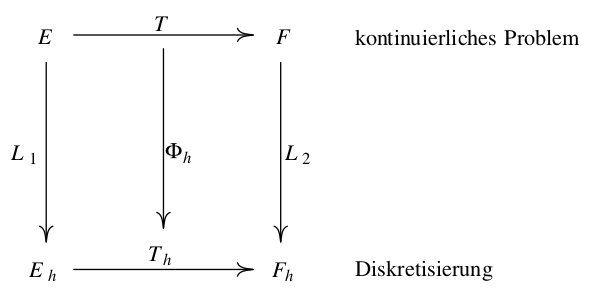
\includegraphics[width=0.45\textwidth]{abstraktkonsistenz.png} \\
	 	Abbildung aus \cite{brokate2016grundwissen} Seite 392
	 \end{figure}
	 Das diskretisierte Problem $ T_h \rho_h = 0  $ heißt genau dann konsistent, wenn für eine analytische Lösung $ \rho^{\star} \in E $ gilt, dass $ \lim\limits_{h \to 0}\lVert \Phi_h(T)L_1\rho^{\star} - L_2T\rho^{\star} \rVert_{F_h} = 0 $.
	 Betrachten wir zunächst in einem Zwischenschritt die Semidiskretisierung (5.3).
	 Die gewählte Herleitung dieser Formulierung soll dabei nahelegen, dass für eine exakte (und glatte) Lösung $ \rho $ die Konsistenz für die Semidiskretisierung erfüllt ist. In oben eingeführter Notation gilt also gerade $ B_h(\rho^{\star},\phi) $ für alle Testfunktionen $ \phi $. Auch wenn es sich bei $ Q_h $ um einen nicht konformen Ansatzraum handelt, ist der Herleitung der Semidiskretisierung dennoch zu entnehmen, dass auch $ B_h(\rho^{\star},\phi_h) $ für alle $ \phi_h \in Q_h $ gilt $(\star)$.  Wichtig ist dabei unter anderem auch die Wahl der numerischen Flussfunktion, der upwind flux erhält aber gerade gewünschten Eigenschaften. 
	 Mehr dazu findet sich in \cite{Har08b}.
	 Für die Zeitdiskretisierung in Form der impliziten Mittelpunktsregel gilt als einstufige Gauß-Quadratur $ \lVert \Phi_h(T)L_1\rho^{\star} - L_2T\rho^{\star} \rVert_{F_h} = O(h^2)$, womit sie insbesondere konsistent ist. \\
	 Daher gilt so für das kombinierte Verfahren, dass eine klassische Lösung $ \rho^{\star} $ somit auch die Volldiskretisierung in obigem Sinne erfüllt. 
\subsubsection{Galerkin Orthogonalität}
Eine direkte Folgerung aus der Konsistenz und $ (\star) $ stellt die Galerkin Orthogonalität dar. Für eine Lösung der Semidiskretisierung $ \rho_h $ und eine analytische Lösung im klassischen Sinne $ \rho^{\star} $ gilt dann nämlich:
\[
 B_h(\rho^{\star}-\rho_h,\phi_h = 0) \quad \forall \phi_h \in \mathcal{Q}_h
\]
\subsubsection{Stabilität und Konvergenz}
Die Stabilität ist bei der numerischen Lösung der Transportgleichung einer der wesentlichen Gründe, weswegen wir das Discontinuous Galerkin Verfahren einem Standard-Finite-Elemente-Ansatz vorziehen. Es zeigt sich nämlich, dass ein normales Finite Elemente Verfahren, wie wir es zuvor bei der Lösung des Potentialströmungsproblems genutzt haben, beim Transportproblem instabil ist. Grund dafür ist, dass $ \lVert q \cdot \nabla \rho_h \rVert $ beliebig groß werden kann. Für die DG-Diskretisierung mit upwind flux kann hingegen gezeigt werden, dass die Lösung des Transportproblems stabil ist. Auf eine theoretische Stabilitätsanalyse möchten wir aber an dieser Stelle verzichten und verweisen z.B. auf \cite{Har08b}.
Ebenso wollen wir bezüglich der Konvergenz des Verfahrens auf entsprechende Literatur verweisen. Wir werden später Konvergenzannahmen stellen und diese in entsprechenden Experimenten verifizieren. In der Literatur finden sich aber auch theoretische Konvergenzbeweise, meist unter Verwendung vielfältiger funktionalanalytischer Grundlagen und unter gewissen Regularitätsvoraussetzungen an die bestimmte Lösung. Die theoretische Betrachtung von Discontinuous Galerkinverfahren ist bereits Gegenstand vielfältiger wissenschaftlicher Arbeiten, aber zugleich ein breites Feld, welches noch lange nicht vollständig erforscht ist. \\
%Im nächsten Abschnitt sollen nun schließlich die Überlegungen der letzten Abschnitte gebündelt werden und wir wollen die Multilevel Monte Carlo Methode bei der speziellen Anwendung auf das Transportproblem betrachten.






%%%%%%%%%%%%%%%%%%%%%%%%%%%%%%%%%
\newpage  % neuer Abschnitt auf neue Seite, kann auch entfallen
%%%%%%%%%%%%%%%%%%%%%%%%%%%%%%%%%
\subsection{Anwendung der MLMC Methode auf das probabilistische Transportproblem}
%%%%%%%%%%%%%%%%%%%%%%%%%%%%%%%%%
\newpage  % neuer Abschnitt auf neue Seite, kann auch entfallen
%%%%%%%%%%%%%%%%%%%%%%%%%%%%%%%%%
\section{Beispiel/Experiment}
\subsection{Konkretes Problem}

\subsection{Ergebnisse}
%%%%%%%%%%%%%%%%%%%%%%%%%%%%%%%%%
\newpage  % neuer Abschnitt auf neue Seite, kann auch entfallen
%%%%%%%%%%%%%%%%%%%%%%%%%%%%%%%%%
\section{Ausblick und Fazit}

  % Literaturverzeichnis (beginnt auf einer ungeraden Seite)
  \newpage

%\begin{thebibliography}{Lam00}
 %Bibiographie
  \bibliographystyle{abbrv}
  \bibliography{References}
%\end{thebibliography}
 
      
  % ggf. hier Tabelle mit Symbolen 
  % (kann auch auf das Inhaltsverzeichnis folgen)

\newpage
  
 \thispagestyle{empty}


\vspace*{8cm}


\section*{Erkl\"arung}

Ich  versichere  wahrheitsgem\"a\ss,  die  Arbeit selbstst\"andig verfasst,  alle  benutzten  Hilfsmittel  vollst\"andig  und  genau  angegeben  und  alles kenntlich  gemacht  zu  haben,  was  aus  Arbeiten  anderer  unver\"andert  oder  mit  Ab\"anderungen entnommen  wurde,  sowie die Satzung  des  KIT  zur  Sicherung guter wissenschaftlicher Praxis in der jeweils g\"ultigen Fassung beachtet zu haben.
\\[2ex] 

\noindent
Ort, den Datum\\[5ex]

% Unterschrift (handgeschrieben)



\end{document}

